
% R00 17.ABR.2018 - Edson Bispo Ferreira. Adaptado por Giovani Fonseca Ravagnani Disperati.
%
%-------------------------------------------------------------------------

\documentclass[
	12pt,				
	oneside,			
	a4paper,			
	english,			
	brazil				
	]{abntex2ppgsi}

% ---s
% Pacotes básicos 

\usepackage[utf8]{inputenc}		% Codificacao do documento (conversão automática dos acentos)
\usepackage{lastpage}			% Usado pela Ficha catalográfica
\usepackage{indentfirst}		      % Indenta o primeiro parágrafo de cada seção.
\usepackage{color}				% Controle das cores
\usepackage{graphicx}		 	% Inclusão de gráficos
\usepackage{microtype} 			% para melhorias de justificação
\usepackage{pdfpages}            %para incluir pdf
\usepackage{algorithm}			%para ilustrações do tipo algoritmo
\usepackage{mdwlist}			%para itens com espaço padrão da abnt
\usepackage[noend]{algpseudocode}			%para ilustrações do tipo algoritmo
\usepackage{quoting}			% pacote de citações (quotes)
\usepackage{setspace}			% pacote singlespace, para citações
\usepackage[Symbol]{upgreek}    %pacote para letras gregas maiúsculas
\usepackage{siunitx}		
\usepackage{multirow}	
		
% ---
% Pacotes de citações
% ---
\usepackage[brazilian,hyperpageref]{backref}	 % Paginas com as citações na bibl
\usepackage[alf]{abntex2cite}	% Citações padrão ABNT

% --- 
% CONFIGURAÇÕES DE PACOTES
% --- 

% ---
% Configurações do pacote backref
% Usado sem a opção hyperpageref de backref
%\renewcommand{\backrefpagesname}{Citado na(s) página(s):~}
% Texto padrão antes do número das páginas
%\renewcommand{\backref}{}
% Define os textos da citação
%\renewcommand*{\backrefalt}[4]{
%	\ifcase #1 %
%		Nenhuma citação no texto.%
%	\or
%		Citado na página #2.%
%	\else
%		Citado #1 vezes nas páginas #2.%
%	\fi}%
% ---

% ---
% Informações de dados para CAPA e FOLHA DE ROSTO
% ---

%-------------------------------------------------------------------------
% Comentário adicional do PPgSI - Informações sobre o ``instituicao'':
%
% Não mexer. Deixar exatamente como está.
%
%-------------------------------------------------------------------------
\instituicao{
	INSTITUTO FEDERAL DE EDUCAÇÃO, CIÊNCIA E TECNOLOGIA 
      \par
      DE SÃO PAULO
	\par
	CAMPUS SÃO PAULO
	\par
	MESTRADO ACADÊMICO EM ENGENHARIA MECÂNICA}


%
%-------------------------------------------------------------------------
\titulo{Análise de falha em rolamentos por análise de vibração com utilização de sensor piezoelétrico polimérico}


%-------------------------------------------------------------------------
\autor{\uppercase{GIOVANI FONSECA RAVAGNANI DISPERATI}}

%-------------------------------------------------------------------------
\local{São Paulo}

%-------------------------------------------------------------------------
\data{2021}


%-------------------------------------------------------------------------
\orientador{Prof. Dr. Wilson Carlos da Silva Junior \newline 
Coorientadora: Profa. Dra. Vanesssa Seriacopi}


\tipotrabalho{Qualificação (Mestrado)}

\preambulo{
%-------------------------------------------------------------------------
%  
%
%
% 
%
%-------------------------------------------------------------------------
. \newline \newline \newline 
%-------------------------------------------------------------------------
Proposta de qualificação apresentada ao Departamento de Engenharia Mecânica do Instituto Federal de Educação, Ciência e Tecnologia de São Paulo, Campus São Paulo como requisito parcial para a obtenção do título de Mestre em Ciências em Engenharia Mecânica. 
%
\newline \newline Área de concentração: Engenharia Mecânica
%-------------------------------------------------------------------------
% 
% 
%
% 
% 
% 
% 
%
%-------------------------------------------------------------------------
\newline \newline \newline .}

\definecolor{blue}{RGB}{41,5,195}

% informações do PDF
\makeatletter
\hypersetup{
     	%pagebackref=true,
		pdftitle={\@title}, 
		pdfauthor={\@author},
    	pdfsubject={\imprimirpreambulo},
	    pdfcreator={LaTeX com abnTeX2 adaptado para o ifsp},
		pdfkeywords={abnt}{latex}{abntex}{abntex2}{qualificação de mestrado}{dissertação de mestrado}{ppgsi}, 
		colorlinks=true,       		% false: boxed links; true: colored links
    	linkcolor=black,          	% color of internal links
    	citecolor=black,        		% color of links to bibliography
    	filecolor=black,      		% color of file links
		urlcolor=black,
		bookmarksdepth=4
}
\makeatother
% --- 

% --- 
% Espaçamentos entre linhas e parágrafos 
% --- 

% O tamanho do parágrafo é dado por:
\setlength{\parindent}{1.25cm}

% Controle do espaçamento entre um parágrafo e outro:
\setlength{\parskip}{0cm}  % tente também \onelineskip
\renewcommand{\baselinestretch}{1.5}

% ---
% compila o indice
% ---
\makeindex
% ---

	% Controlar linhas orfas e viuvas
  \clubpenalty10000
  \widowpenalty10000
  \displaywidowpenalty10000

% ----
% Início do documento
% ----
\begin{document}

% Retira espaço extra obsoleto entre as frases.
\frenchspacing 

% ----------------------------------------------------------
% ELEMENTOS PRÉ-TEXTUAIS
% ----------------------------------------------------------
% \pretextual

% ---
% Capa
% ---

\imprimircapa
% ---

% ---
% Folha de rosto
% ---
\imprimirfolhaderosto
% ---



% ---
% RESUMOS
% ---

% resumo em português
\setlength{\absparsep}{18pt} % ajusta o espaçamento dos parágrafos do resumo
\begin{resumo}

%-------------------------------------------------------------------------

%\begin{flushleft}
%DISPERATI, Giovani Fonseca Ravagnani. \imprimirtitulo. \imprimirdata. \pageref{LastPage} f. Proposta de qualificação (Mestrado em Ciências) %– Departamento de Engenharia Mecânica, Instituto Federal de Educação, Ciência e Tecnologia de São Paulo, São Paulo, 2018.
%\end{flushleft}

O fluoreto de polivinilideno, conhecido pela sigla PVDF, é um polímero com características piezo e piroelétricas, além de alta estabilidade e resistência química e física que, aliadas ao fácil processamento desse material, o tornam um excelente elemento para uso tecnológico. PVDF é um material semicristalino flexível, de baixo custo de fabricação e fácil de usinar. Seu uso passa por diversas aplicações, desde sensores até a construção de tubos e dutos para o transporte de água ultrapura. Sua cristalização ocorre em pelo menos quatro fases distintas, alfa, beta, gama e delta, sendo que a fase beta é caracterizada por apresentar os comportamentos piezo e piroelétricos já mencionados.
Dadas estas características, trabalhos têm sido desenvolvidos utilizando filmes feitos deste material como sensores para manutenção preditiva baseada em análise de vibração. O tema deste trabalho surge da proposta de avaliar o filme PVDF como um sensor aplicado na detecção de falhas em mancais de rolamentos, um dos elementos de máquina mais comuns, uma vez que o PVDF possui caracteríticas que o tornam candidato a ser uuma alternativa aos sensores habitualmente utilizados para este fim. O PVDF tem menor custo em relação a estes e, portanto, o componente econômico é a motivação para esta investigação.
O objetivo deste trabalho é adquirir um sinal de vibração utilizando um sensor PVDF, para que seja realizada a detecção de falhas em mancais em um software supervisório com aplicações de manutenção preditiva. Com base nos sinais captados deste sensor, será possível avaliar a viabilidade de um sistema de sensor PVDF para monitoramento das condições dos mancais. Para tanto, foi construída uma bancada experimental na qual o sensor PVDF é acoplado aos mancais escolhidos como objeto de estudo. Um circuito também foi construído para condicionar e amplificar o sinal de saída do sensor, de forma que ele possa ser capturado por um sistema de aquisição de dados. A partir desta saída espera-se encontrar o melhor posicionamento do sensor para capturar os sinais de falha, a fim de diferenciar os sinais de um rolamento autocompensador de rolos com as seguintes falhas: desgaste da pista do anel interno, desgaste da pista do anel externo e desgaste no elemento rotativo. Espera-se que isso culmine na possibilidade de determinar um nível de alarme indicativo de uma situação de pré-falha.


Palavras-chaves: Manutenção preditiva. Rolamentos. Análise de vibração. PVDF.
\end{resumo}

% resumo em inglês

\begin{resumo}[Abstract]
\begin{otherlanguage*}{english}

Polyvinylidene fluoride, known by the acronym PVDF, is a polymer with piezo and pyroelectric characteristics, in addition to high chemical and physical stability and resistance that, combined with the easy processing of this material, make it an excellent element for technological use. PVDF is a flexible semi-crystalline material, low in manufacturing cost and easy to machine. Its use goes through a variety of applications, from sensors to the construction of pipes and ducts for the transport of ultrapure water. Its crystallization occurs in at least four distinct phases, alpha, beta, gamma and delta, and the beta phase is characterized by having the aforementioned piezo and pyroelectric behaviors.
Given these characteristics, works have been developed using films made of this material as sensors for predictive maintenance based on vibration analysis. The theme of this work arises from the proposal to evaluate the PVDF film as a sensor applied in the detection of failures in bearing housings, one of the most common machine elements, since the PVDF has characteristics that make it a candidate to be an alternative to the ceramic sensors customarily used for this purpose. The PVDF also has a much lower cost compared to them and this economic component, therefore, is the motivation for this investigation.
The objective of this work is to acquire a vibration signal using a PVDF sensor, so that the detection of bearing failures in a supervisory software with predictive maintenance applications is performed. Based on the signals captured from this sensor, it will be possible to assess the viability of a PVDF sensor system for monitoring bearing conditions. For this purpose, an experimental bench was built in which the PVDF sensor is coupled to the bearings chosen as the object of study. A circuit was also built-in order to condition and amplify the sensor's output signal, so that it can be captured by a data acquisition system. From this output it is expected to find the best positioning of the sensor to capture the failure signals, in order to differentiate signals from a spherical roller bearing with the following failures: wear of the inner ring raceway, wear on the outer ring raceway and wear on the rolling element. It is expected that this culminates in the possibility of determining an alarm level indicative of a pre-failure situation.


Keywords: Predictive Maintenance. Bearings. Vibration analysis. PVDF.
\end{otherlanguage*}
\end{resumo}

% ---
% ---
% inserir lista de figuras
% ---
\pdfbookmark[0]{\listfigurename}{lof}
\listoffigures*
\cleardoublepage
% ---
% inserir lista de tabelas
% ---
\pdfbookmark[0]{\listtablename}{lot}
\listoftables*
\cleardoublepage
% ---

% ---
% inserir lista de abreviaturas e siglas
% ---
%-------------------------------------------------------------------------
% Comentário adicional do PPgSI - Informações sobre ``Lista de abreviaturas 
% e siglas'': 
%
% Opcional.
% Uma vez que se deseja usar, é necessário manter padrão e consistência no
% trabalho inteiro.
% Se usar: inserir em ordem alfabética.
%
%-------------------------------------------------------------------------
\begin{siglas}
  \item[PVDF] Fluoreto de Polivinilideno
  \item[BPFI] Ball Pass Frequency Inner Race
  \item[BPFO] Ball Pass Frequency Outer Race
  \item[BSF] Ball Spin Frequency 
\end{siglas}
% ---

% ---
% inserir lista de símbolos
% ---

\begin{simbolos}
  \item[$ \alpha $] Letra grega Alfa
  \item[$ \beta $] Letra grega Beta
  \item[$ \gamma $] Letra grega Gama
  \item[$ \delta $] Letra grega Delta
  \item[$ \theta $] Letra grega Teta  
  \item[$ \mu $] Letra grega Mi  
  \item[$ \sigma $] Letra grega Sigma
  \item[$ \upphi $] Letra grega Phi maiúscula
  \item[$ \omega $] Letra grega Omega
  \item[\SI{}{\metre}] Metro  
  \item[\SI{}{\micro\metre}] Micrometro
  \item[$ \in $] Pertence
\end{simbolos}
% ---

% ---
% inserir o sumario
% ---
\pdfbookmark[0]{\contentsname}{toc}
\tableofcontents*
\cleardoublepage
% ---


% ----------------------------------------------------------
% ELEMENTOS TEXTUAIS
% ----------------------------------------------------------
\textual



%-------------------------------------------------------------------------

\chapter{Introdução}
De acordo com a Confederação Nacional das Indústrias, o setor industrial representa, em outubro de 2019, 21,6\% do produto interno bruto do Brasil. Também responde por 70,8\% das exportações nacionais, 67,4\% dos investimentos empresariais em pesquisa  e 34,2\% dos tributos federais, excetuando-se receitas previdenciárias (CNI, 2019). 

Neste âmbito destaca-se, portanto, a importância da manutenção como ferramenta econômica para a indústria e, consequentemente, para a economia nacional. Processos de manutenção preventiva, ou de manutenção preditiva, tem por finalidade mitigar a ocorrência de falhas catastróficas, diminuindo perdas econômicas por paradas inesperadas ou, mesmo, por custos de seguridade social decorrentes de acidentes de trabalho causados por máquinário defeituoso.

De acordo com a NBR 5462, manutenção preventiva é uma "manutenção efetuada em intervalos pré-determinados, ou de acordo com critérios prescritos, destinada a reduzir a probabilidade de falha ou a degradação do funcionamento de um item" (NBR 5462, p. 7). Já a manutenção preditiva, é definida como uma manutenção que "permite garantir uma qualidade de serviço desejada, com base na aplicação sistemática de técnicas de análise, utilizando-se meios de supervisão centralizados ou de amostragem, para reduzir ao mínimo a manutenção preventiva e diminuir a manutenção corretiva" (NBR 5462, p. 7). 

Para que o processo de manutenção preditiva possa ocorrer é necessário, como estabelecido pela NBR 5462, a aplicação sistemática de técnicas de análise. Para tanto, a coleta de informações relativas ao estado dos elementos de máquina é pré-requisito, sendo, para isto, utilizado uma vasta gama de sensores com diferentes propósitos e especificidades afim de aferir os mais distintos parâmetros destes elementos. 

Dentre os diversos elementos de máquina um dos mais comuns são os rolamentos, com utilização em virtualmente todas as áreas da indústria. Esta categoria de elemento de máquina, portanto, foi escolhida como objeto de testes e estudo afim de verificar a viabilidade de uma tecnologia  de sensores com finalidade, dentre outras, de manutenção preditiva: o filme de fluoreto de polivinilideno. 

Tem-se vários tipos de polímeros, sendo os de maior interesse tecnológico os eletroativos, capazes de realizar a conversão entre energia elétrica e energia mecânica. Em outras palavras, estes polímeros apresentam alteração em seu tamanho e/ou forma quando são sujeitos a um campo elétrico. Alguns  materiais dentro desta família apresentam também outro efeito: geram um sinal elétrico quando sujeitos a uma força. Devido a estas caraterísticas, os polímeros eletroativos são ideais para a aplicação em sensores e atuadores, onde por sua baixa massa especifica, substituem sistemas pesados e complexos, possibilitando projetos de novas aplicações devido a uma mais simples implementação e miniaturização (Bar-Cohen, 2002).

O fluoreto de polivinilideno, conhecido pela sigla PVDF, apresenta características piezo e piroelétricas, além de elevada estabilidade e resistência química e física que, combinadas ao fácil processamento deste material, o tornam um excelente elemento para utilização tecnológica. O PVDF é um material semicristalino flexível e de baixo custo de fabricação, de fácil usinagem, múltiplas aplicações e com grande resistência química (Fukada, 2000; Lang, 2006). O PVDF foi descoberto em 1969 por Kawai, sendo um material novo com utilização perpassando uma variedade de , desde sensores para medição de vibrações mecânicas até a construção de canos e dutos para transporte de água ultrapura. A sua cristalização ocorre em pelo menos quatro fases distintas, $\alpha$, $\beta$, $\gamma$ e $\delta$ (Silva, 2009). A fase $\beta$ é caracterizada por possuir comportamento piezo e piroelétrico (Wisnieski, 2002).

O tema deste trabalho surge da proposta de se avaliar o filme PVDF como sensor de vibração com finalidades de manutenção preditiva, em particular, aqui, aplicado a falhas de rolamentos, uma vez que este sensor possui baixo custo e, desta forma, mostra-se como possível alternativa aos acelerômetros cerâmicos costumeiramente utilizados para esta finalidade. O componente econômico, portanto, se faz basilar neste trabalho. 

Dadas estas características do material, o filme PVDF foi utilizado como sensor de vibração. Uma vez que a tensão de saída é proporcional a força mecânica aplicada é possível avaliar a severidade da vibração sofrida pelo rolamento e, assim, realizar-se a detecção de padrões que indiquem o comprometimento do elemento, bem como apontar qual o problema em potencial.

%Sabendo-se que as suas propriedades de piezoeletricidade surgem após esforço mecânico, verifica-se a possibilidade de utilização deste como alternativa aos acelerômetros cerâmicos normalmente utilizados para análise de vibração.    

Esta tensão então, a partir de sua aquisição e conversão por um conversor analógico-digital, pode ser transmitida e estes dados armazenados através de um software de aquisição de dados, para que se realize posterior análise. Uma vez que o filme PVDF está sujeito a interferências por vibrações externas, sinais de alta frequência e outros fatores, bem como tendem a possuir baixa voltagem de saída, é necessário o condicionamento deste sinal com um circuito eletrônico específico para tanto. 

%Desta forma, o sensor filme PVDF foi utilizado pois possui as supracitadas características que o tornam tecnologicamente e economicamente viável para a aplicação proposta. 

Portanto, foi construído um encapsulamento para o sensor, bem como um circuito de condicionamento do sinal e um sistema de software para aquisição de dados afim de análise das informações capturadas pelo sensor durante os testes na bancada experimental, também construída para este trabalho. 

A fim de testar , foi construída bancada experimental com mancais de rolamentos de rolos, da empresa NSK, acoplados a um eixo em um motoredutor cedido por empresa parceira WEG/Cestari. 

Espera-se que, a partir dos experimentos, possa se obter uma resposta inicial quanto a viabilidade de utilização do filme PVDF para fins de manutenção preditiva.

%A análise de vibração é uma das técnicas de manutenção preditiva empregadas na indústria; Nesta, é possível que se realize a medição do estado do componente, sendo este considerado um método efetivo para monitoração de elementos rolantes - incluindo-se, aí, rolamentos (Kern et al, 2014). 


\chapter{Objetivos}

\section{\textbf {Geral}}

Em relação aos objetivos do trabalho, visa-se, de forma geral, a aquisição de sinal de vibração, com a utilização de sensor PVDF, para que seja realizada a detecção de falhas em rolamentos em um sistema supervisor com aplicações de manutenção preditiva. A partir disto será possível avaliar a viabilidade de um sistema de sensores PVDF para monitoramento das condições de rolamentos em maquinários, afim de possibilitar uma alternativa mais barata em relação aos sensores atualmente utilizados para este fim.

\section{\textbf {Específicos}}

Os objetivos específicos do trabalho podem ser sumarizados em:

\begin{itemize}
	\item Construir uma bancada experimental em que o sensor PVDF possa ser acoplado aos rolamentos escolhidos.
	\item Realizar o tratamento do sinal de saída do sensor, de forma a ser capturado por um sistema de aquisição de dados.
	\item Desenvolver um sistema de aquisição de dados para o sensor PVDF, quando trabalhando com sinais de falha de rolamento.
	\item Desenvolver um sistema de análise dos dados capturados.
	\item Diferenciar um sinal de falha de rolamento de esfera com uma, com as seguintes falhas: 1 - desgaste da pista do anel interno, 2 - desgaste na pista do anel externo e 3 - desgaste no elemento rolante.
	\item Determinar um nível de alarme, indicativo de uma situação pré falha.
	\item Encontrar o melhor posicionamento do sensor para captar os sinais de falha.
\end{itemize}

\chapter{Revisão Bibliográfica}
%Neste capítulo serão abordados os conceitos essenciais que embasam este projeto, a saber: os fundamentos da manutenção preditiva; os fundamentos, aplicações e revisão de falhas de mancais de rolamentos; os fundamentos de vibração mecânicas; a aquisição de sinais vibracionais para análise preditiva de falhas nos mancais de rolamentos; os fundamentos da aquisição, análise de sinais e algoritmos para processamento destes sinais aquisitados, que será implementada no software supervisor.

Neste capítulo são abordados os principais conceitos que embasam o projeto, a saber: os fundamentos da manutenção preditiva, tópico focal de nosso projeto; os fundamentos, aplicações e revisão de falhas de mancais de rolamentos, em particular considerando os que serão abordados nos experimentos práticos que serão conduzidos; os fundamentos de vibração mecânicas, afim de embasar a aquisição de sinais vibracionais para análise preditiva de falhas nos mancais de rolamentos; fundamentos da aquisição, análise de sinais e algoritmos para processamento destes sinais aquisitados, que será implementada no software supervisor.

Também será feita uma revisão acerca do fenômeno piezoelétrico presente no PVDF, material escolhido para os sensores utilizados na aquisição dos sinais vibracionais dos mancais de rolamentos que serão utilizados neste trabalho. 


\section{\textbf{Manutenção}}
Todo e qualquer meio no qual se pretenda fabricar alguma coisa precisa de meios que permitam a produção (Nepomuceno, 1989), estes meios podem variar desde instrumentos simples, como tesouras, agulhas e novelos de lã, até maquinário industrial de alta complexidade. Em qualquer destes casos sempre surgem as questões de desgaste, enguiços, quebras e fraturas, dentre outros possíveis problemas. Portanto, em toda atividade produtiva  há necessidade de manutenção, sem a qual a produção colapsa (Nepomuceno, 1989).

	Usualmente classifica-se a manutenção em três formas distintas: corretiva, preventiva e preditiva (Holanda, 2016). 

	A manutenção corretiva, também conhecida por manutenção reativa, diz respeito a prática correspondente a primeira geração das técnicas de manutenção. A manutenção corretiva foi utilizada desde as primeiras industrias até, aproximadamente, o final dos anos 40 do século XX – período em que a indústria era pouco mecanizada e com maquinário comparativamente mais simples. Seu princípio é a utilização do equipamento até sua quebra, sendo apenas então realizado o reparo (Holanda, 2016). 
	
	Entretanto, de acordo com Holanda, 2016	

\begin{citacao}

	Este tipo de manutenção baseada no tempo, porém, não elimina a possibilidade de ocorrência de falhas inesperadas no período, visto que a taxa de falha de 	muitas máquinas não é melhorada com a substituição regular de partes gastas. Pelo contrário, frequentemente a confiança nas máquinas recém-trabalhadas é 		reduzida, temporariamente, devido à interferência humana. (Holanda, 2016)

\end{citacao}

Assim, faz-se necessária uma forma de manutenção que particularize cada máquina, de forma a avaliar sistematicamente suas condições. Isto começa a ocorrer nos 70 do século XX, com os avanços da automação e elevação das exigências de confiabilidade e disponibilidade. A este método de manutenção chama-se de manutenção preditiva. (Holanda, 2016).  


\subsection{\textbf{Manutenção preditiva}}

Para Nepomuceno, 1989, p.41 a manutenção preditiva tem por finalidade 

\begin{citacao}

[...]estabelecer, numa instalação industrial qualquer, quais são os parâmetros que devem ser escolhidos em cada tipo de máquina ou equipamento, em função das informações que as alterações de tais parâmetros sobre o estado mecânico de um determinado componente (pistões, dilatação, rolamentos, vasão, particulado, etc.). Em base a tais informações, a análise dos mesmos permitirá que sejam tomadas providências visando evitar estragos de monta ou mesmo situações catastróficas irreversíveis. (Nepomuceno, 1989, p.41)

\end{citacao}

Assim, portanto, “a manutenção preditiva visa realizar manutenção somente quando as instalações precisarem dela” (Slack, 2008, p.645). 

De acordo com Nepomuceno, 1989, quando se estuda a manutenção preditiva esta, em uma análise superficial, parece demasiadamente dispendiosa, há a evidente necessidade de medição e análise de diversos parâmetros e, para tanto, é necessários instrumentos de análise e medição, além de alteração de processos convencionais de medição e controle da condição do maquinário. Entretanto, ainda de acordo com Nepomuceno, 1989, analisando mais detalhadamente esta questão percebe-se que a manutenção preditiva apresenta vantagens que a tornam economicamente viável. Dentre outras, cita-se: 


\begin{itemize}
	\item Reparos se tornam menos custosos que uma quebra de maquinário e consequente interrupção da produção;
	\item A rejeição é diminuída devido ao constante ajuste do equipamento, acarretando, portanto, em menor perda de materiais;
	\item Equipamentos reserva podem, em muitos casos, ser eliminados;
	\item Controle de peças e materiais sobressalentes, diminuindo sensivelmente os custos de estoque;
	\item Controle de componentes mais substituídos bem como de equipamentos que apresentam maior número de defeitos permite o rastreamento da origem dos problemas: se no material, equipamento ou operadores;
	\item Diminuição da ociosidade produtiva acarretada por falhas;
	\item Redução de 15\% a 20\% do custo global em comparação aos métodos clássicos de manutenção, quando computados os custos de peças, materiais e mão-de-obra;
	\item Diminuição sensível, ou mesmo eliminação, da manutenção corretiva;
\end{itemize}

Além destes argumentos Holanda, 2016, chama a atenção para o fato de a manutenção preditiva ter como benefício colateral a capacidade de determinação automática do Tempo Médio Entre Falhas, MTBF (\textit{Mean Time Between Failures}). Segundo Holanda, 2016

\begin{citacao}
Esse indicador fornece os subsídios para se determinar o tempo mais efetivo em termos de custo para substituir o maquinário, ao invés de continuar a absorver altos custos de manutenção. No momento em que o MTBF atinge o ponto no qual os custos de manutenção e de operação do equipamento excederem os custos da substituição, a máquina deve ser substituída. (Holanda, 2016)
\end{citacao}

Para a condução de um processo de manutenção preditiva existem diferentes técnicas. Holanda (2016) cita como as principais técnicas: 
\begin{itemize}
	\item termografia, técnica que, através de temperatura, realiza a formação de imagens térmicas para atuação no diagnóstico de falhas; 
	\item análise de lubrificantes, técnica que verifica fatores que possam ser danosos a operação do equipamento através da análise de viscosidade, acidez, teor da água dentre outros; 
	\item ultrassom, técnica que permite a detecção de descontinuidades internas através da propagação de ondas através do equipamento; 
	\item líquido penetrante, técnica que possibilita a verificação de descontinuidades superficiais tais como trincas, poros e dobras; 
	\item análise de vibrações, técnica que permite o monitoramento do desenvolvimento de falhas em maquinário e peças através de medições de suas assinaturas vibracionais. 
\end{itemize}

Cada elemento de máquina possui características particulares que influenciam os métodos de manutenção preditiva adotados. No caso dos mancais de rolamentos estes geram vibrações mesmo quando geometricamente perfeitos, uma vez que possuem um número finito de elementos rolantes afim de suportar a carga. Ainda, quando ocorre um defeito em um dos componentes de um mancal de rolamentos, há aumento considerável nos níveis de vibração do mesmo. (Barilli, 2013, p. 8)

Assim, a manutenção preditiva baseada em análise de vibrações, aplicada à mancais de rolamentos, será abordada em maiores detalhes por se tratar da técnica escolhida dadas as características dos rolamentos, bem como do sensor objeto de estudo deste trabalho.

\section{\textbf{Análise de vibrações}}

Para que se possa abordar as técnicas de manutenção preditiva baseada em análise de vibrações faz-se necessário, primeiramente, um breve entendimento relativo ao fenômeno das vibrações mecânicas. 

Segundo Rao, 2008, p.5

\begin{citacao}
A maioria das atividades humanas envolve vibração de uma forma ou outra. Por exemplo, ouvimos porque nossos tímpanos vibram, e vemos porque as ondas de luz sofrem vibração. A respiração está associada à vibração dos pulmões, e andar envolve movimento oscilatório (periódicos de pernas e mãos). Falamos devido ao movimento oscilatório da laringe (e da língua). (Rao, 2008)
\end{citacao}

Ainda, segundo Holanda, 2016, as vibrações mecânicas são fenômenos que acontecem constantemente na natureza e no cotidiano humano. Holanda define vibração mecânica como

\begin{citacao}
\,[...]um tipo de movimento no qual se considera uma massa reduzida a um ponto submetido a uma força. A ação dessa força obriga o ponto a executar um movimento oscilatório. Para que o movimento oscilatório do ponto se constitua numa vibração, ele deverá percorrer uma trajetória denominada trajetória completa ou ciclo, conhecida pelo nome de período de oscilação. (Holanda, 2016)
\end{citacao}

Nepomuceno, 1989, p.229 afirma que as vibrações mecânicas são fenômenos observados quando uma partícula realiza um movimento entorno uma posição de equilíbrio. Assim, quando há troca de energia cinética em energia potencial e vice-versa, ocorre a vibração. Quando um corpo oscila em períodos determinados ao redor de uma posição de equilíbrio, caracteriza-se este movimento como Movimento Harmônico, forma mais simples que a vibração pode se apresentar (Holanda, 2016). Holanda, 2016, apresenta como exemplo disto o movimento do pêndulo de um relógio, que oscila da máxima posição à direita até a máxima posição à esquerda, passando pelo ponto central de equilíbrio. 

%Este movimento é graficamente representado como uma senoide, conforme mostrado na Figura 16, abaixo.

%\begin{figure}[!htb]
%\centering
%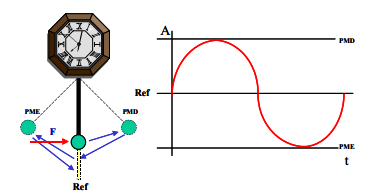
\includegraphics{Figura16}
%\caption {Representação do movimento harmônico simples através do pêndulo de um relógio. A senóide representa graficamente o movimento. Retirado de Holanda, 2016, p.20}
%\label{Figura16}
%\end{figure}

Ressalta-se que o tempo que a massa demora para realizar uma oscilação, ou movimento harmônico simples, é chamado de período. Uma oscilação por segundo, ou um ciclo por segundo, CPS, constitui uma medida de frequência denominada Hertz (Nepomuceno, 1989). 

Em relação ao movimento harmônico simples, ou oscilação, Nepomuceno, 1989, p.233 ressalta que

\begin{citacao}
Nos casos práticos, existem inúmeros osciladores mecânicos que são dispositivos que dão origem a oscilações simples, principalmente às amplitudes pequenas ou então fornecem combinações de oscilações. É importante observar que todo e qualquer sistema que obedeça a Lei de Hooke é apto a oferecer tal tipo de vibrações. (Nepomuceno, 1989, p.233)
\end{citacao}

Para que se mensure os níveis de vibração, utiliza-se parâmetros expressos em termos de deslocamento, velocidade e aceleração (Holanda, 2016). Segundo Holanda, 2016, p. 21 \textit{apud} Kardec e Nascif, 2009, p.244 todos os três parâmetros representam “o quanto o equipamento está vibrando”. 

Além disso, estes parâmetros possuem amplitude, frequência e fase. A amplitude, A, se relaciona com a quantidade de energia contida no sinal vibratório, ou seja, a severidade do movimento, sendo medida em milímetros (mm). Pode ser tomada em forma de deslocamento, velocidade e aceleração. A frequência, f, conforme anteriormente mencionado, é representada em Hertz e indica o número de vezes em que ocorre um ciclo completo de movimento. Já a fase, $\upphi$, representa “o ângulo inicial do argumento da função senoidal que descreve o movimento harmônico” (Holanda, 2016, p. 22).

Já em relação às formas de mensuração, o Deslocamento é medido em micrometros (\SI{}{\micro\metre}). De acordo com Holanda, 2016, p.21 o deslocamento pode ser medido pelo nível de distanciamento do ponto relativo à sua posição de repouso, sendo a “unidade mais óbvia para se mensurar a vibração, pois é aquela que mais se aproxima da ideia de oscilação em torno de um ponto médio”. O deslocamento é recomendado para medições abaixo de 10Hz (Holanda, 2016). A fórmula abaixo representa o deslocamento, x:

\[x = A \,sen (\omega t + \upphi)\]

A velocidade, por sua vez, é medida em milímetros por segundo ($mm/s$). O deslocamento implica na existência de uma velocidade que, por sua vez, pode ser variável. A função de velocidade, v, é dada por:

\[v = A\omega \,cos (\omega t + \upphi)\]

Holanda, 2016, p.21 afirma que a velocidade de vibração é parâmetro “menos representativo para componentes tanto de baixa como de alta frequência, sendo o parâmetro normalmente escolhido para avaliação da severidade de vibração entre 10 Hz e 1000 Hz”.

A aceleração, por sua vez, é medida em metros por segundo ao quadrado ($m/s^{2}$). Com velocidade variável, implica-se a existência de uma aceleração no movimento. A fórmula que representa a aceleração, a, é:

\[a = -A^{2} \omega \,sen (\omega t + \upphi)\]

Limitando-se o escopo de abrangência, este fenômeno das vibrações, na engenharia, é um item de alta relevância para estudo visto que os efeitos das vibrações podem ser nocivos, ou mesmo catastróficos, ao se considerar maquinário industrial. 

Fatores como desgaste precoce de elementos mecânicos e falhas por fadiga causadas por movimentos cíclicos podem ser mensurados ao monitorar a assinatura vibracional dos componentes de máquina. A partir disto são aplicadas, então, técnicas específicas que permitam a adequada mensuração do estado dos componentes. 


\subsection{\textbf{Técnicas de análise de vibrações}}

Esclarecidos os conceitos  fundamentais relativos as vibrações mecânicas, faz-se necessário entender como as vibrações podem ser medidas e analisadas sob a ótica do interesse tecnológico na manutenção preditiva. 

Nepomuceno, 1989, p.206 afirma que a medida e monitoramento da vibração é uma das atividades de manutenção preditiva que apresenta melhores resultados. Mesquita et. al, 2002, afirmam que análise destas vibrações pode se dar nos domínios do tempo, da frequência e no domínio conjunto tempo-frequência.

Em relação à análise no domínio do tempo, Segundo Spamer, 2009, p.62 apud Holanda, 2016, p.22 a amplitude de vibração em função do tempo pode ser medida em valores de pico a pico, valor de pico e valor RMS. Meola, 2005, afirma que o valor de pico a pico sinaliza a excursão máxima da onda, medida relevante para definição de quando um elemento da máquina atinge valores críticos. Já o valor de pico, de acordo com Meola, 2005, indica níveis máximos de sinais transientes, sem considerar a cronologia da onda. O valor médio, por sua vez, indica o quanto o sinal está deslocado quanto à sua referência tendo pouca relevância quanto ao monitoramento da vibração. 

Já o valor RMS, ou eficaz, é, de acordo com Meola, 2005, p.9

\begin{citacao}
\,[...]uma das medidas mais importantes de amplitude, uma vez que quantifica a energia que está diretamente ligado ao fenômeno estudado, no caso é um indicativo do poder destrutivo da vibração. É muito utilizado como parâmetro global para determinação de níveis de alerta e alarme usados em procedimentos de manutenção preditiva.
\end{citacao}

A relação entre os níveis de pico, o nível médio, é dada por:

\[Nivel \, M\acute{e}dio = \frac{1}{T} \int_{0}^{T} x(t)dt \]

Já o nível eficaz, ou nível RMS, de um sinal harmônico é dado por:

\[Nivel \, RMS = \sqrt{ \frac{1}{T} \int_{0}^{T} x^{2}(t)dt }  \]

A Figura~\ref{RelacaoSinalHarmonico}, abaixo, exemplifica a relação estes níveis.

\begin{figure}[!htb]
\centering
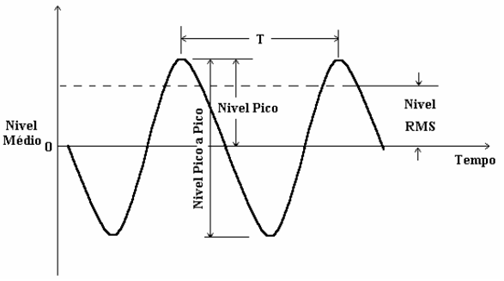
\includegraphics[width=\textwidth,height=\textheight,keepaspectratio]{Figura17}
\caption {Representação dos níveis de um sinal harmônico. Retirado de Meola, 2005.}
\label{RelacaoSinalHarmonico}
\end{figure}

De acordo com Tandon, 1999 apud Meola, 2005, os métodos mais comuns de detecção de falhas no domínio do tempo são o nível RMS e o Fator de Crista, que representa a razão entre o valor de pico e o valor RMS de aceleração. O Fator de Crista, FC, considera a variação do pico e do valor RMS. Considerando-se mancais de rolamentos, Meola afirma que a diferença entre estes é de aproximadamente 3dB, dada por:

\[20log_{10} \left ( \frac{Nivel \,Pico}{Nivel \, RMS} \right ) \]

Esta diferença aumenta progressivamente com o surgimento de defeitos, até atingir valor aproximado de 18dB quando, devido ao desgaste geral do rolamento, tal diferença volta a diminuir (Meola, 2005). Assim, ao retornar para aproximadamente 3dB a falha é iminente e o rolamento deverá ser trocado. 

A Figura~\ref{RelacaoPicoaPicoeRMS}, abaixo, demonstra esta relação entre os valores de Pico e RMS.  

\begin{figure}[!htb]
\centering
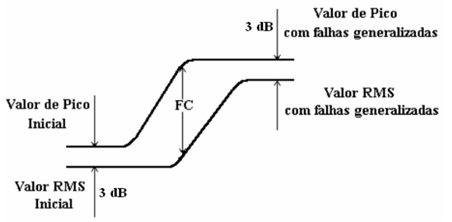
\includegraphics[width=\textwidth,height=\textheight,keepaspectratio]{Figura18}
\caption {Relação entre os valores de Pico e RMS com o desgaste progressivo de rolamentos. Retirado de Meola, 2005.}
\label{RelacaoPicoaPicoeRMS}
\end{figure}	

Já a Figura~\ref{FatorCrista}, abaixo, demonstra o comportamento do Fator de Crista no tempo com o desgaste do rolamento.

\begin{figure}[!htb]
\centering
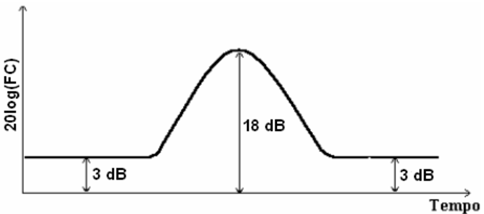
\includegraphics[width=\textwidth,height=\textheight,keepaspectratio]{Figura19}
\caption {Fator de Crista no tempo.}
\label{FatorCrista}
\end{figure}	

Outro relevante método para detecção de falhas é a curtose. Neste, os momentos estatísticos são utilizados para descrever o comportamento de variáveis aleatórias. A curtose é utilizada na detecção de falhas incipientes em rolamentos. Segundo Mesquita et al., 2002

\begin{citacao}
A Densidade de Probabilidade do sinal de aceleração de um rolamento também pode ser usada para a detecção de falhas em rolamentos. Um rolamento em boas condições possui uma distribuição Gaussiana de aceleração, enquanto que o rolamento defeituoso produz uma distribuição não-gaussiana devido ao aumento no número dos altos níveis de aceleração.
Vários momentos estatísticos podem ser usados para indicar a forma da densidade de probabilidade. Dyer e Stewart propuseram o Fator de Curtose, que é o quarto momento estatístico, normalizado em relação ao desvio padrão elevado a quarta potência.
\end{citacao}

A curtose é descrita da seguinte forma:

\[K = \frac{ \int_{-\infty}^{+\infty} (x - \overline{x})^{4}p(x)dx } {\sigma^{4}} \]

Onde $p(x)$ é a função de densidade de probabilidade e $\overline{x}$ o valor médio do sinal de vibração \textit{x(t)}. Segundo Mesquita et al. 2002, o fator de curtose para mancais em bom estado é igual a três, sendo que este valor tende a aumentar conforme o rolamento se deteriora. 

Os métodos descritos, de análise de falhas no domínio do tempo, são capazes de indicar o surgimento da falha. Entretanto, tais métodos não são capazes de apontar onde se localiza tal falha. Para isto, faz-se necessário a utilização de análise no domínio da frequência. 

Tendo em vista que os mancais possuem frequências características de defeitos, espera-se que, ao apresentar falhas em seus componentes, tais falhas possam ser determinadas a partir das frequências por elas geradas. Desta forma, técnicas de análise espectral, tal como a transformada rápida de Fourier, podem mostrar onde se localiza o defeito. Mesquita et. al, 2002, entretanto, apontam para o fato de que podem ocorrer pequenos deslizamentos entre as pistas, o que pode ocasionar desvios nas frequências de defeitos em relação ao que se espera. Portanto, recomendam que tais frequências características sejam utilizadas como referência. Além disso, ainda, Mesquita et. al, 2002, atentam para o fato de que tais frequências podem ser mascaradas por outros elementos da máquina, dificultando a identificação das frequências de defeitos através de análise espectral tradicional.


\section{\textbf{Fundamentos e aplicações de rolamentos}}
Rolamentos são dispositivos para transmissão de movimentos rotacionais ou lineares, com finalidade de redução de atrito entre partes móveis (Santos et al., 2007). Rolamentos são compostos, geralmente, de dois anéis, elementos rolantes e uma gaiola, sendo classificados como rolamentos radiais ou axiais, dependendo da direção da carga principal (NSK, 2018). Adicionalmente, os rolamentos são classificados como rolamentos de esferas e rolamentos de rolos, em função do tipo de elemento rolante, e segregados quanto seus propósitos específicos (NSK, 2018).

A Figura~\ref{ComponentesRolamentos}, abaixo, demonstra os componentes de um rolamento de uma carreira esferas e suas dimensões. 

\begin{figure}[!htb]
\centering
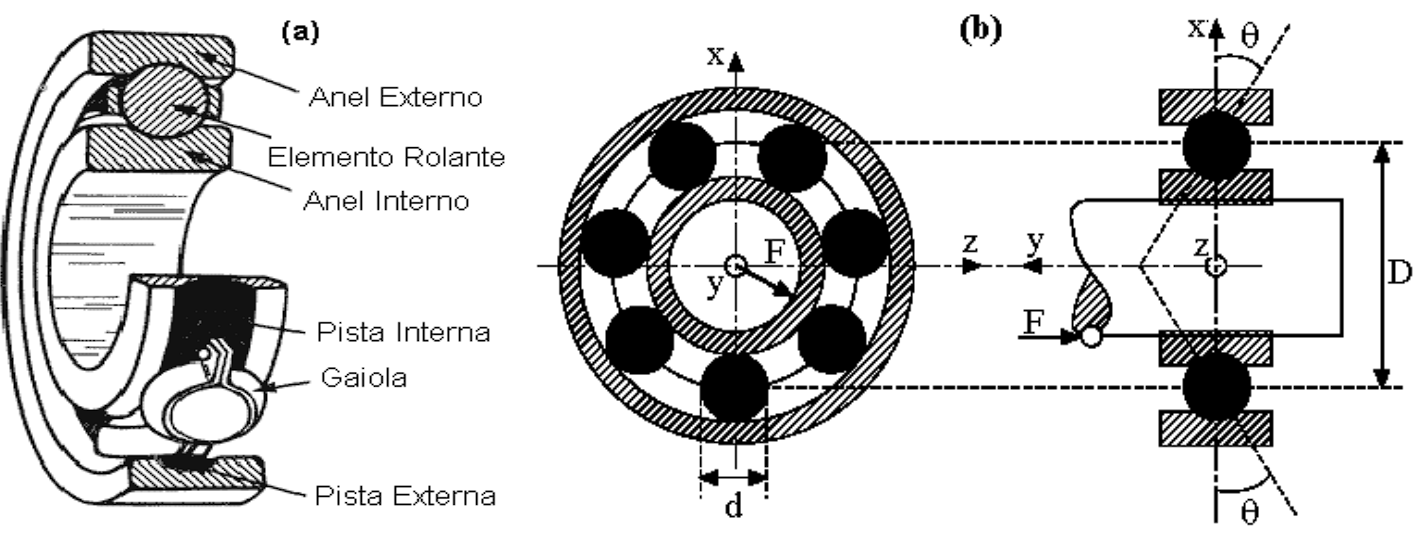
\includegraphics[width=\textwidth,height=\textheight,keepaspectratio]{Figura1}
\caption{a) Componentes de um rolamento. (b) Dimensões do rolamento. Mesquita et al. 2002 apud Santos et al. 2017}
\label{ComponentesRolamentos}
\end{figure}

Segundo a NSK (2018), 

\begin{citacao}
Atualmente, os rolamentos são uma das peças de máquina mais comumente usadas porque seu movimento de rolamento torna quase todos os movimentos mais fáceis e ajudam a reduzir a fricção. Rolamentos têm duas funções-chave: transferem movimento, isto é, suportam e guiam componentes que giram um em relação ao outro; transmitem forças.
\end{citacao}

Em comparação aos mancais de deslizamento, os rolamentos apresentam vantagens como: torque de partido e atrito baixos, com diferença entre torque de partida de partida e torque de funcionamento pequenos; grande padronização internacional, facilitando sua substituição; dentre outras (NSK, 2018).

%A seguir apresenta-se uma revisão sobre tipos de rolamentos, suas principais características, propriedades e tipos de falhas.

\subsection{\textbf{Tipos de rolamentos}}

Os rolamentos, de forma semelhante às rodas, são componentes que podem rolar  e que servem para redução de atrito entre eles e a superfície (Abecom, 2019). Existem distintos tipos de rolamentos, dentre os quais cita-se:

\begin{itemize}
	\item Rolamentos de rolos cilíndricos, constituídos por uma carreira de rolos em uma gaiola
	\item Rolamentos de rolos cônicos, contrítudos por pistas de anel interno e externo, cônicas e rolos cônicos
	\item Rolamentos autocompensadores, que possuem duas carreiras de esferas ou rolos com uma pista esférica comum no anel externo e duas pistas no anel interno 	
	\item Rolamentos rígidos de esfera, que são rolamentos versáteis de concepção simples e tipo não separáveis
	\item Rolamentos de esfera de contato angular, que possui pistas nos anéis interno e externo
	\item Rolamentos axiais de esferas, que são são projetados para cargas axiais]
\end{itemize}

Cada tipo de rolamento possui suas aplicações e a escolha de rolamento depende de uma série de fatores específicos, tais como a carga a ser suportada, a velocidade de funcionamento, temperatura de trabalho, folga interna, alinhamento e desalinhamento do eixo, espaço disponível, dentre outros. 


\subsection{\textbf{Processos de fabricação de rolamentos}}

Nos rolamentos usualmente segrega-se o processo de fabricação em: fabricação dos anéis interno e externo; fabricação das esferas; fabricação das gaiolas e, por fim, montagem (Dos Santos et al., 2017).   

As esferas, ou rolos, são feitas a partir de barras de aço cortadas em comprimentos específicos. Um processo de forjamento destes fragmentos de barra confere às peças o formato desejado, mas ainda com rebarbas. É realizado, então, o desbaste destas rebarbas. Após o processo de desbaste as esferas passam por tratamento térmico de têmpera. Por fim, é realizado o polimento. 

Os anéis interno e externo, por sua vez, são criados pelos mesmos processos, a saber: forjamento, torneamento, tratamento térmico, polimento e super-acabamento. No  primeiro processo, forjamento, os lingotes de aço são aquecidos e, através de prensagem, são formados os anéis interno e externo em cada movimento da prensa. Os processos decorrem, portanto, simultaneamente e no mesmo equipamento. Após o forjamento, se dá o processo de torneamento. Neste, o torneamento do anel interno e externo se dá pelos mesmos passos. Primeiramente é torneada uma face lateral, a largura do anel. Em seguida, a outra face lateral é torneada. O próximo passo do processamento do anel é o torneamento do perfil da pista e largura. Simultaneamente é usinado o chanfro do anel. Em sequência ao processo de torneamento, se dá o tratamento térmico dos anéis por tempera, onde estes são aquecidos a temperaturas superiores aos 800ºC, bruscamente resfriados em óleo, reaquecidos em temperaturas de 150ºC e resfriados ao ar. Por fim, há o processo de acabamento onde processos abrasivos e de polimento são utilizados para atingir acabamento fino e exatidão de dimensão das peças (Dos Santos et al., 2017). 

A Figura~\ref{FiguraProcessoFabricacao}, abaixo, demonstra o fluxo de ordenação destes processos acima descritos.
\begin{figure}[!htb]
\centering
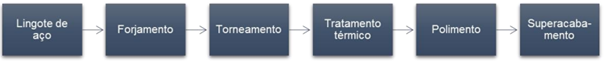
\includegraphics[width=\textwidth,height=\textheight,keepaspectratio]{Figura2}
\caption{a) Processo de fabricação dos anéis internos e externos. Retirado de Dos Santos et al., 2017.}
\label{FiguraProcessoFabricacao}
\end{figure}

As gaiolas, por sua vez, são produzidas com lâminas de aço que recebem a forma de anéis planos através de estampagem, sendo, então, prensadas para receber forma ondulada afim de manter as esferas na posição, feitos os furos para rebites e tratamento térmico da peça. (Dos Santos et al., 2017).
 
Com todas as partes produzidas é realizada, então, a montagem do rolamento. Primeiro, os anéis interno e externo são colocados concentricamente na linha de produção com as esferas preenchendo os espaços entre estes. O tamanho dos elementos rolantes se dá por calculo a partir do diâmetro da ranhura do anel interno. Estes são, então, uniformemente organizados por um divisor e uma metade da gaiola é adicionada. Em sequência outra máquina adiciona a metade restante da gaiola e finaliza-se, assim, a montagem da peça. (Santos et al., 2017). 


\subsection{\textbf{Carga e vida útil de rolamentos}}

A vida nominal básica de um rolamento é dada na norma ISO 281:2007, que também específica os métodos de cálculo de classificação de carga dinâmica básica. Em relação a classificação de carga dinâmica básica, C, esta é utilizada para cálculos que envolvem rolamentos dinamicamente tensionados (SKF, 2019). Tal classificação expressa a carga do rolamento que resultará em uma vida nominal básica, L10, de um milhão de revoluções (SKF , 2019). O valor de C é usualmente encontrado nos catálogos referência das fabricantes.   

Para a vida nominal básica temos na ISO 281:2007 que:

\[L_{10}= \left ( \frac{C}{P} \right )^{p}  \]

Onde $L_{10}$ é a vida nominal básica, com 90\% de confiabilidade, expressa em milhões de revoluções; C é a classificação da carga dinâmica básica, em kN; P é a carga dinâmica equivalente do rolamento, em kN; e, por fim, p é o expoente da equação de vida, que é 3 para rolamentos de esferas e 10/3 para rolamentos de rolos (SKF, 2019).

Se a velocidade for constante, por sua vez, torna-se preferível calcular a vida útil em horas de operação (SKF, 2019). Para tanto, utiliza-se :

\[L_{10h}= \frac{10^{6}}{60_{n}}L_{10}\]

Onde $L_{10h}$ é a vida nominal básica, com 90\% de confiabilidade, expressa em horas operacionais e n é a velocidade de rotação, em rotações por minuto. 
Para que se possa calcular a vida nominal básica de um rolamento usando as classificações de cargas dinâmicas básicas é necessário, entretanto, que esta seja convertida, primeiramente, em carga dinâmica equivalente do rolamento. A carga dinâmica equivalente do rolamento, P, é “definida como uma carga hipotética, com magnitude e direção constantes, que atua radialmente em rolamentos radiais e axial e centralmente em rolamentos axiais” (SKF, 2019). Esta carga hipotética teria influência na vida do rolamento igual às cargas reais que o rolamento é submetido.

Para os rolamentos híbridos, por sua vez, as mesmas vidas nominais podem ser utilizadas. Segundo a SKF, 2019

\begin{citacao}
Experiências e testes diversos mostram que, em aplicações de máquinas-ferramentas normais, a vida útil de um rolamento híbrido é significativamente maior do que a vida útil de um rolamento com elementos rolantes de aço. A vida útil estendida de rolamentos híbridos deve-se à dureza, baixa densidade e acabamento superficial dos elementos rolantes. A baixa densidade minimiza a carga interna das forças centrífuga e de inércia, enquanto a maior dureza torna os elementos rolantes menos suscetíveis ao desgaste. Seu acabamento superficial permite que o rolamento otimize os efeitos do lubrificante. (SKF, 2019)
\end{citacao}

Em relação à carga mínima requerida, rolamentos que operem em alta velocidade e/ou estejam sujeitos a acelerações bruscas, forças de inércia dos elementos rolamentos e atrito do lubrificante podem ser prejudiciais aos elementos rolantes e as pistas (SKF, 2019). Assim, para o adequado funcionamento os rolamentos devem estar sujeitos a uma carga mínima de 0,01C para rolamentos de esferas e 0,02C para rolamentos de rolos. 

Por fim, em determinadas aplicações as condições operacionais, tais como a magnitude, sentido das cargas, velocidades, temperaturas e lubrificação são variáveis (SKF, 2019). O cálculo de vida útil em condições operacionais variáveis não pode ser calculado antes da redução do espectro de carga e do ciclo de trabalho. Para tanto, cada nível de carga pode ser acumulado e o espectro de carga reduzido a um histograma de blocos constantes de carga (SKF, 2019).

Para o cálculo de vida útil em condições variáveis, utiliza-se:

\[L_{10}= \frac{1}{ \frac{U_{1}}{L_{10 \,1}} + \frac{U_{2}}{L_{10 \,2}} + \frac{U_{3}}{L_{10 \,3}} + ...}\]

Onde $L_{10}$ é a vida nominal básica, com 90\% de confiabilidade, $L_{10 \,1}$, $L_{10 \,2}$ são as vidas nominais básicas, com 90\% de confiabilidade, em condições constantes 1, 2 e, por fim, $U_{1}$, $U_{2}$ são as frações, que devem totalizar 1, do ciclo de vida sob as condições 1, 2 etc. De acordo com SKF, 2019

\begin{citacao}
Dentro de cada intervalo de trabalho, a carga e as condições operacionais do rolamento podem ter um valor médio constante. O número de horas de operação ou revoluções esperadas de cada intervalo de trabalho que mostram a fração de vida necessária para essa condição de carga específica. Portanto, se ${N_{1}}$ for igual ao número de rotações necessárias na condição de carga ${P_{1}}$, e N for o número esperado de rotações para concluir todos os ciclos de carga variável, então a fração de ciclo ${U_{1} = N_{1} / N}$ é utilizada pela condição de carga ${P_{1}}$, que possui uma vida útil calculada de ${L_{10 \,1}}$. (SKF, 2019)
\end{citacao}


\subsection{\textbf{Falhas em rolamentos}}

Quando há correto manuseio dos rolamentos, usualmente estes podem ser utilizados por longos períodos de tempo antes de surgirem sinais de fadiga. Entretanto, devido a seleção incorreta do rolamento, lubrificação inadequada ou mesmo falhas de manuseio ou de condição de serviço, podem ocorrer falhas prematuras (NSK, 2014).

Ainda que a operação se dê de forma adequada, entretanto, a ação das tensões cíclicas de cisalhamento causa o aparecimento de microfissuras que, em sua maioria, surgem em pontos de pouca resistência, ou onde o material é anisotrópico  ou em pontos onde ocorrem inclusões de materiais não metálicos. Assim, com o tempo, estas microfissuras evoluem para a superfície da pista onde surgirão microtrincas que evoluem gradativamente (Harris, 1991; Juvinall e Marshek, 1991).

Dentre as falhas mais comuns em rolamentos temos as seguintes: escamamento, descascamento, arranhadura, escorregamento, fraturas, trinca e lascamento, gaiola danificada, impressões, \textit{pitting}, desgaste, corrosão por atrito, falso brinel, deslizamento, superaquecimento, corrosão eletrolítica, oxidação e corrosão, falha na instalação e alteração na coloração.

%manchas e asperezas superficiais,  desgaste regular,  amassados e arranhamentos, deformação, manchas e descorolação.

Escamamento é o processo em que regiões com textura áspera e grosseira são formadas por separação de pequenas partes de material dos rolamentos devido a fadiga do mesmo. Dentre as possíveis causas estão: carga excessiva, falha na instalação, carga de momento elevada, contaminação por partículas ou por água, lubrificação dificiente ou folga inapropiada (NSK, 2014). A Figura~\ref{escamemento_nsk} mostra anéis internos de rolamentos com escamamento. 

\begin{figure}[H]
\centering
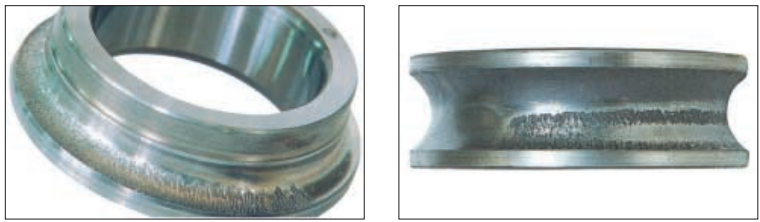
\includegraphics[width=\textwidth,height=\textheight,keepaspectratio]{escamamento_nsk}
\caption {Anéis internos de rolamentos apresentando escamamento. Retirado de NSK, 2014.}
\label{escamemento_nsk}
\end{figure}

Descascamento, por sua vez, é o processo em que a superfície da pista começa a descascar, logo sem seguida sendo percebidas ondulações. Dentre as possíveis causas para esta falha estão: excesso de carga ou manejo inadequado, montagem inadequada, precisão incorreta no eixo ou alojamento, folga insuficiente, contaminação, oxidação, lubrificação inadequada ou mesmo queda de dureza devido temperaturas altas anormais (NSK, 2014). A Figura~\ref{descascamento_nsk} mostra uma pista com descascamento.

\begin{figure}[H]
\centering
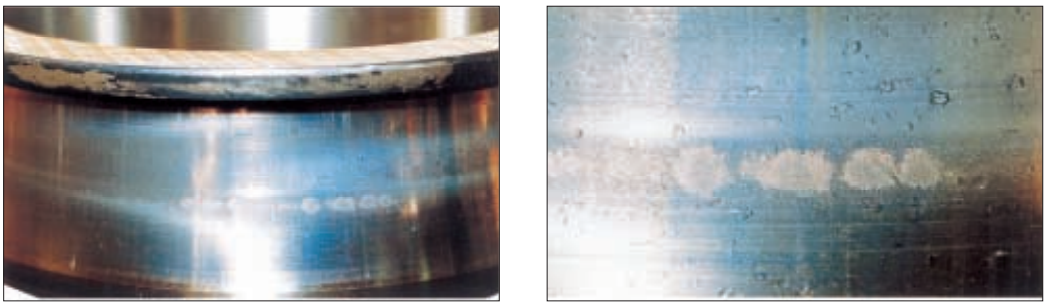
\includegraphics[width=\textwidth,height=\textheight,keepaspectratio]{descascamento_nsk}
\caption {Pista de rolamento com descascamento. Retirado de NSK, 2014.}
\label{descascamento_nsk}
\end{figure}

Amassados e arranhaduras são riscos durante a montagem, arranhamentos em razão de objetos estranhos e duros, além de amassados superficiais devido a impactos. As causas são presença de objetos estranhos, penetração por impacto no lado descascado, quedas e choques devido manejo inadequado além de montagem desalinhada (NSK, 2014). A Figura~\ref{arranhaduras_nsk} mostra amassados e arranhaduras. 

\begin{figure}[H]
\centering
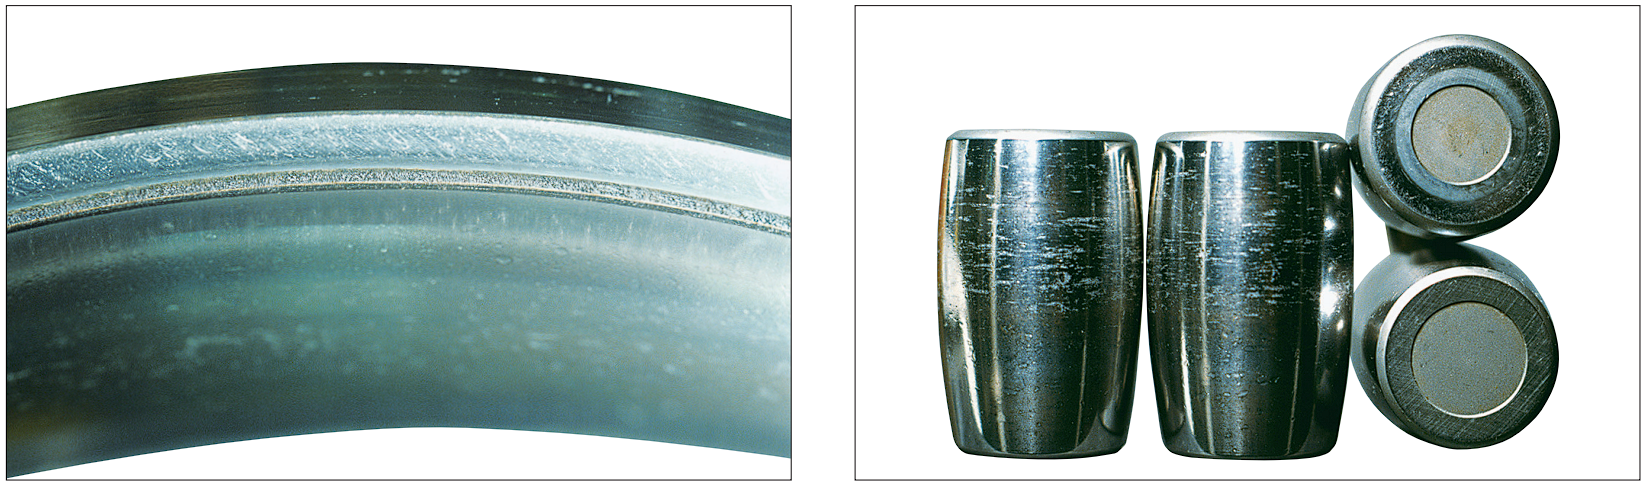
\includegraphics[width=\textwidth,height=\textheight,keepaspectratio]{arranhaduras_nsk}
\caption {Rolamentos com amassados e arranhaduras. Retirado de NSK, 2014.}
\label{arranhaduras_nsk}
\end{figure}

Escorregamento refere-se ao dano causado na superficíe das pistas e elementos rolantes causados pelo rompimento do filme de lubrificação. As causas são alta velocidade e baixa carga, acelerações e desacelerações repentinas, lubrificante inadequado e entrada de água. A Figura~\ref{escorregamento_nsk} mostra um anel interno e um anel externo que sofreram escorregamento. 

\begin{figure}[H]
\centering
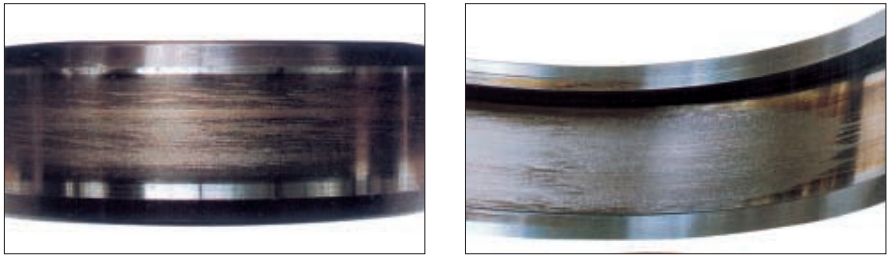
\includegraphics[width=\textwidth,height=\textheight,keepaspectratio]{escorregamento_nsk}
\caption {Aneís interno e externo com danos por escorregamento. Retirado de NSK, 2014.}
\label{escorregamento_nsk}
\end{figure}

Fraturas, por sua vez, referem-se à corpos rolantes partidos, anel interno ou externo partidos ou, mesmo, a gaiolas danificadas. As causas usualmente são carga de anormal na gaiola por problema na instalação ou deficiência de lubrificantes, avanço do processo de escamamento ou, ainda, carga excessiva de choque e desenvolvimento de trinca de fricção. A Figura~\ref{fraturas_nsk} mostra três exemplos de anéis interno e um de anel externo com fraturas. 

\begin{figure}[H]
\centering
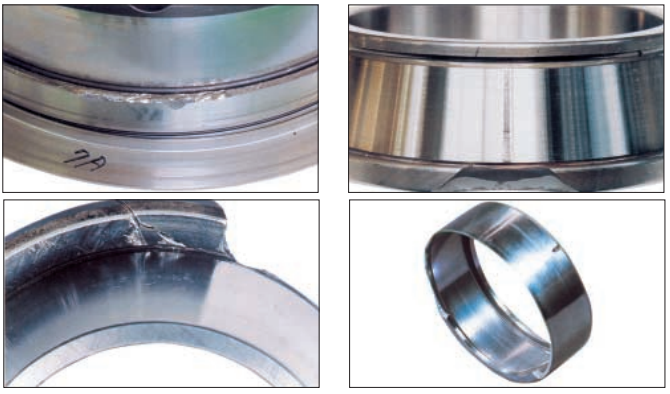
\includegraphics[width=\textwidth,height=\textheight,keepaspectratio]{fraturas_nsk}
\caption {Anéis internos e anel externo com fraturas. Retirado de NSK, 2014.}
\label{fraturas_nsk}
\end{figure}


O aparecimento de trinca e lascamento se dá quando ocorre um descascamento localizado, nisto surgem pequenas trincas ou lascamentos, dentre as possíveis causas para esta falha estão excessivas cargas de choque, excessiva interferência, formação de grandes descascamentos, formação de descascamento por atritos, encostos ou chanfros inadequados ou, ainda, manejo inadequado (NSK, 2014). A Figura~\ref{trinca_nsk} mostra rolamento com trincas e lascamentos. 

\begin{figure}[H]
\centering
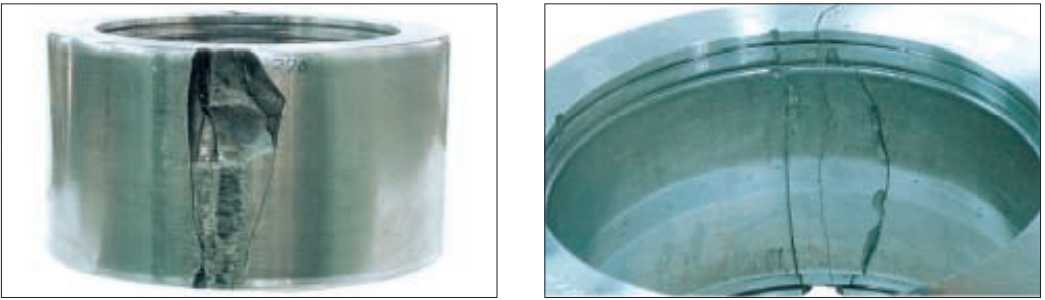
\includegraphics[width=\textwidth,height=\textheight,keepaspectratio]{trinca_nsk}
\caption {Rolamento com lasca e trincas. Retirado de NSK, 2014.}
\label{trinca_nsk}
\end{figure}

Em relação a gaiola danificada, esta falha acontece quando há fratura do pilar da gaiola. Isto resulta na quebra da gaiola. As possíveis causas para esta falha são falha de instalação, carga de momento elevada, altas rotações ou excesso de variação de rotação, lubrificação inadequada, impacto com objetos estranhos, vibração excessiva ou, mesmo, aumento anormal da temperatura (NSK, 2014). A Figura~\ref{gaiola_nsk} mostra gaiolas danificadas. 

\begin{figure}[H]
\centering
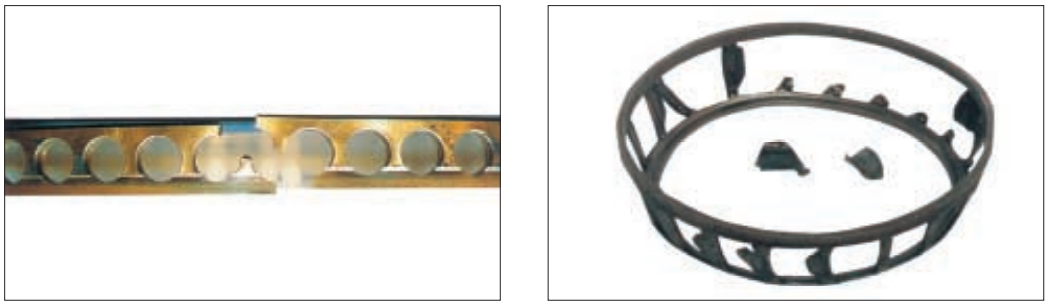
\includegraphics[width=\textwidth,height=\textheight,keepaspectratio]{gaiola_nsk}
\caption {Gaiolas danificadas. Retirado de NSK, 2014.}
\label{gaiola_nsk}
\end{figure}

Impressões referem-se ao ao contato de particulas com os elementos rolantes, marcando a superfície da pista e dos próprios elementos. Dentre as possíveis causas estão a contaminação por partículas, carga excerssiva ou impactos durante transporte e instalação. A Figura ~\ref{impressoes_nsk} mostra um anel interno e elementos rolantes do tipo rolos com impressões.

\begin{figure}[H]
\centering
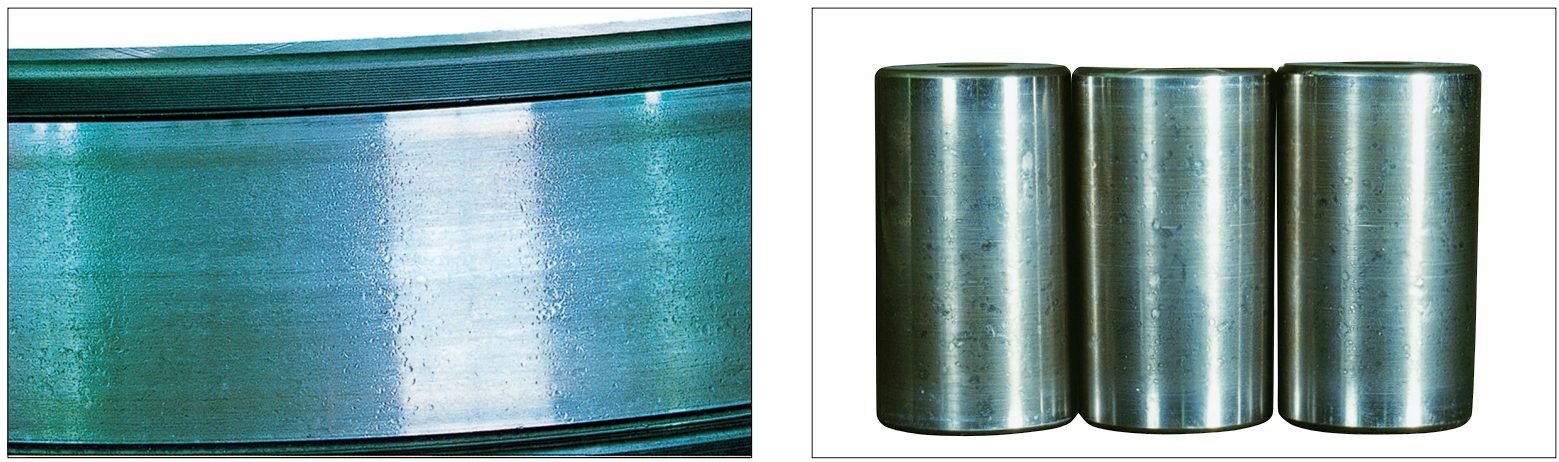
\includegraphics[width=\textwidth,height=\textheight,keepaspectratio]{impressoes_nsk}
\caption {Anel interno e rolos com impressões. Retirado de NSK, 2014.}
\label{impressoes_nsk}
\end{figure}

Outra falha comum, \textit{Pitting}, ocorre quando a superfície se torna áspera e os elementos apresentam uma coloração fosca. As causas incluem lubrificação inadequada, presença de partículas estranhas, afinamento das pontas dos corpos rolantes em razão de um desalinhamento, ruptura da película lubrificante devido excesso de cargas axiais (NSK, 2014). A Figura~\ref{pitting_nsk} apresenta um anel interno e uma esfera com \textit{pitting}.

\begin{figure}[H]
\centering
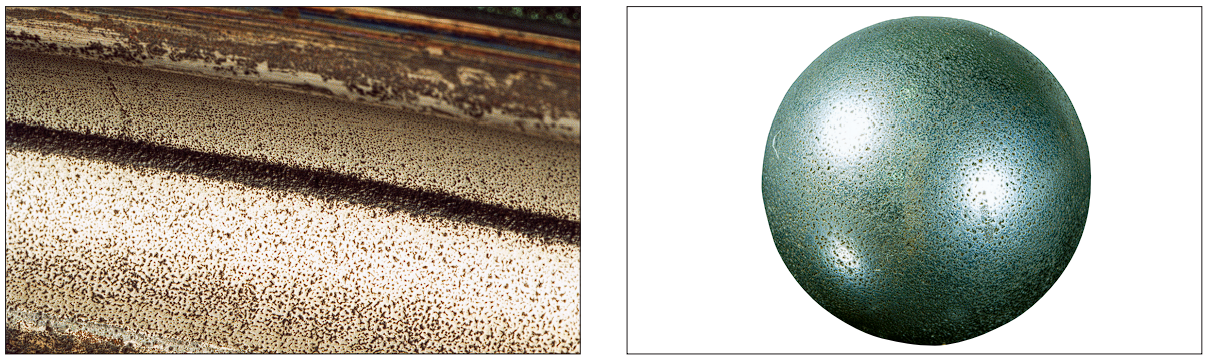
\includegraphics[width=\textwidth,height=\textheight,keepaspectratio]{pitting_nsk}
\caption {Anel interno e esfera com \textit{pitting}. Retirado de NSK, 2014.}
\label{pitting_nsk}
\end{figure}

Desgaste, por sua vez, é o processo em que as superfícies se desgastam e produzem uma deformação dimensional. O desgaste frequentemente acompanha rugosidade e riscos. As causas para o desgaste incluem presença de partículas estranhas no lubrificante, lubrificação inadequada e rolos afinados nas pontas (NSK, 2014). A Figura ~\ref{desgaste_nsk} mostra pistas de rolamentos com desgaste.

\begin{figure}[H]
\centering
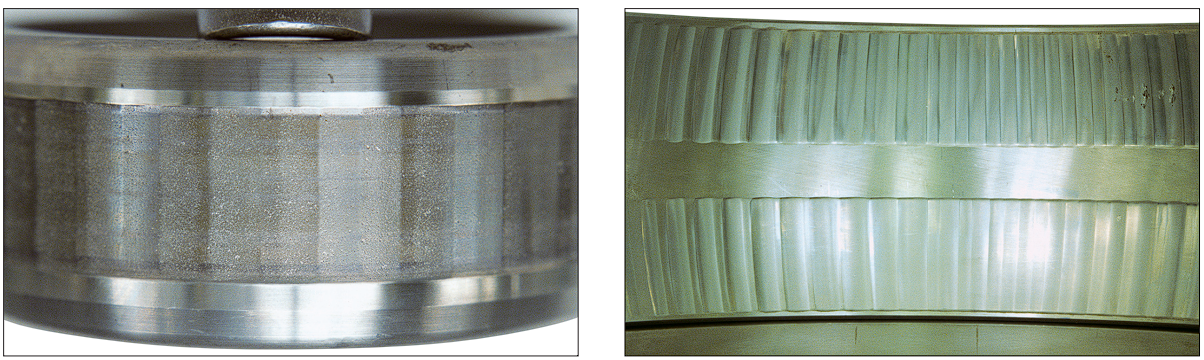
\includegraphics[width=\textwidth,height=\textheight,keepaspectratio]{desgaste_nsk}
\caption {Anel interno e externo com desgaste. Retirado de NSK, 2014.}
\label{desgaste_nsk}
\end{figure}

%Padrões de desgaste, por sua vez, ocorrem pela ação dos corpos rolantes ao longo das superfícies das pistas. Causas para esta falha incluem eixo ou alojamento com precisão insuficiente, instalação imprópria, insuficiência de rigidez do eixo ou alojamento, ou, mesmo, giro do eixo causado pelo excesso de folga interna do rolamento (NSK, 2014). A Figura ~\ref{desgaste_nsk} mostra padrões de desgastes nas pistas do rolamento.

%\begin{figure}[!htb]
%\centering
%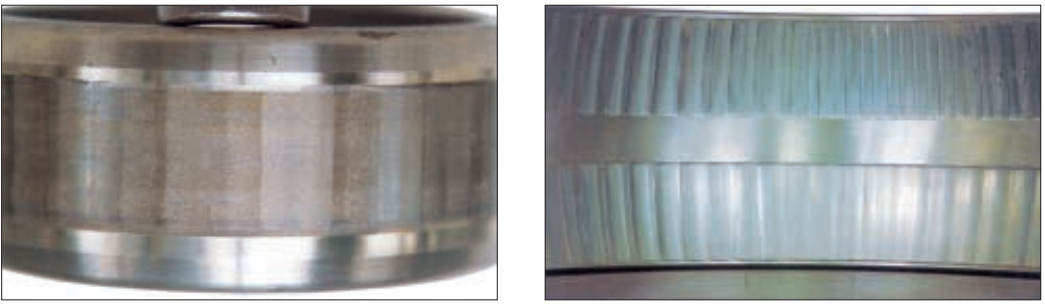
\includegraphics[width=\textwidth,height=\textheight,keepaspectratio]{desgaste_irregular_nsk}
%\caption {Rolamentos com padrões de desgaste. Retirado de NSK, 2014.}
%\label{desgaste_nsk}
%\end{figure}


Corrosão por contato, ou corrosão por atrito, é um tipo de desgaste por raspagem corrosiva. Há duas formas de corrosão por atrito: no primeiro, forma-se um pó de óxido sobre as superfícies de contato; no segundo, ocorre afundamentos nas pistas ao longo do passo dos corpos rolantes. As causas para estas falhas incluem ângulo de oscilação pequeno do rolamento, lubrificação insuficiente, cargas variáveis, vibração durante transporte e, ainda, interferência insuficiente (NSK, 2014). A Figura~\ref{corrosao_nsk} mostra corrosão por contato.

\begin{figure}[H]
\centering
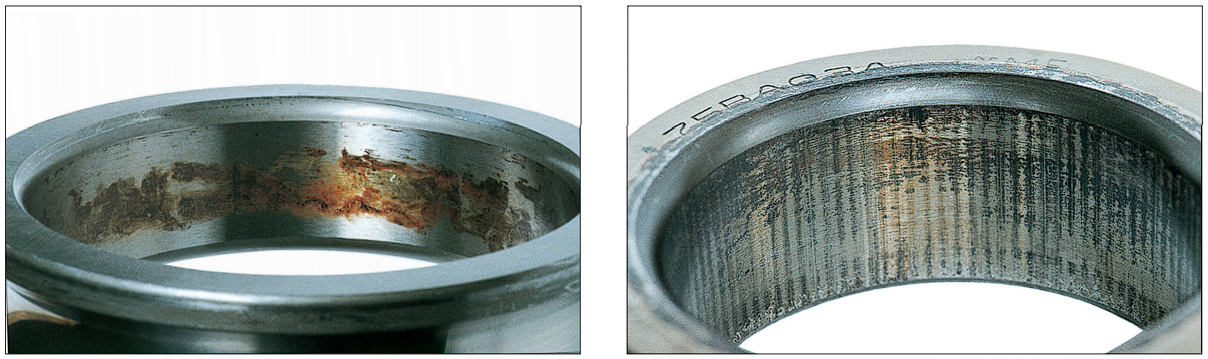
\includegraphics[width=\textwidth,height=\textheight,keepaspectratio]{corrosao_nsk}
\caption {Rolamentos com corrosão por contato. Retirado de NSK, 2014.}
\label{corrosao_nsk}
\end{figure}

Falso brinel refere-se ao esmagamento nas pistas e elementos rolantes por vibração ou oscilação entre os pontos de contato. Dentre as possíveis causas estão lubrificante deficiente ou pequena amplitude no movimento de oscilação (NSK, 2014). A Figura~\ref{esmagamento_nsk} mostra um anel interno e um externo com esmagamento em suas pistas.

\begin{figure}[H]
\centering
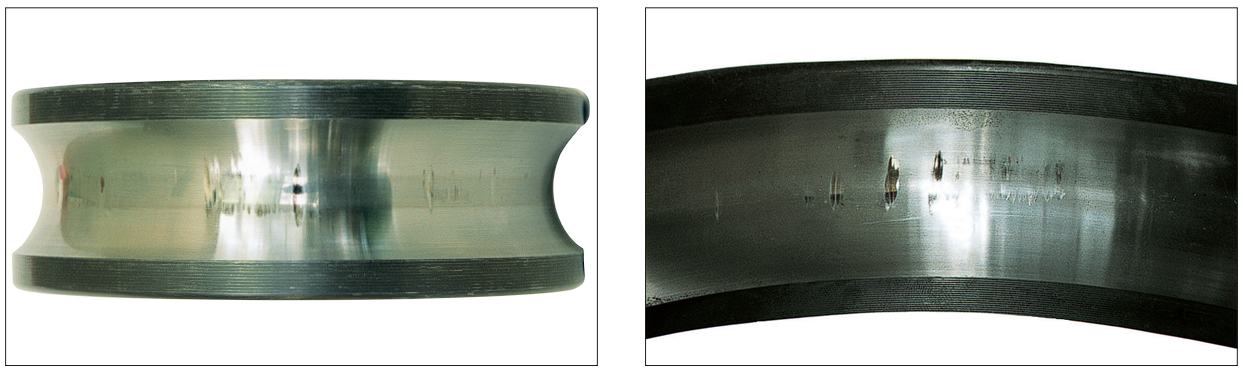
\includegraphics[width=\textwidth,height=\textheight,keepaspectratio]{esmagamento_nsk}
\caption {Pistas com esmagamento. Retirado de NSK, 2014.}
\label{esmagamento_nsk}
\end{figure}

Deformação de deslizamento é acompanhada de superfícies brilhantes ou de superfícies descoloridas no anel interno ou externo, também podendo ocorrer desgaste abrasivo. As causas são interferência insuficiente na seção sem brilho, bucha de montagem não fixada apropriadamente, aumento anormal de temperatura ou, ainda, cargas excessivas (NSK, 2014). A Figura~\ref{deslizamento_nsk} mostra deformação de deslizamento.

\begin{figure}[H]
\centering
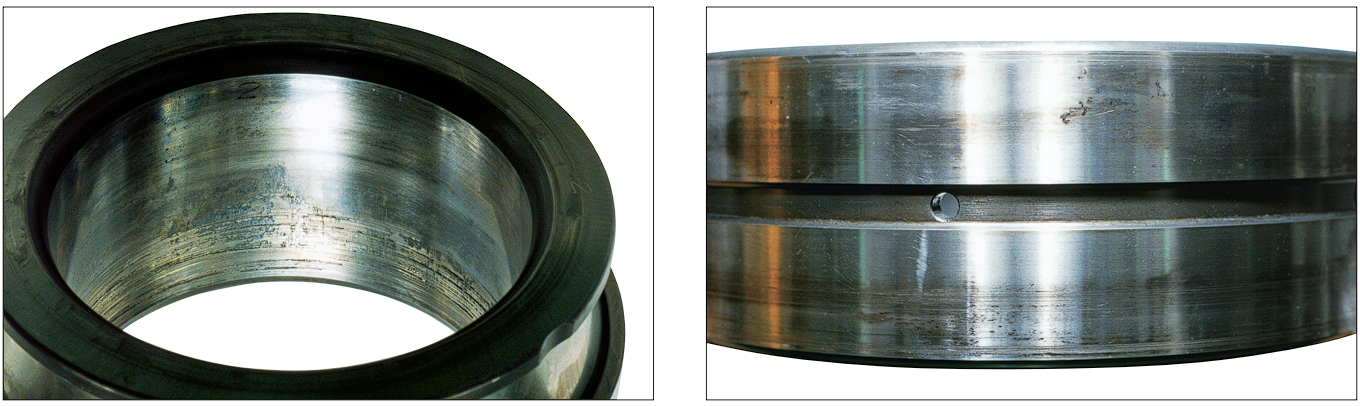
\includegraphics[width=\textwidth,height=\textheight,keepaspectratio]{deslizamento_nsk}
\caption {Deformação de deslizamento. NSK, 2014.}
\label{deslizamento_nsk}
\end{figure}


Superaquecimento, por sua vez, diz respeito ao processo em que o rolamento se aquece e descolora, eventualmente travando. Dentre as possíveis causas para esta falha estão folga insuficiente no rolamento, incluindo-se folgas que diminuem em razão de deformações locais, lubrificação insuficiente ou imprópria, cargas excessivas ou ainda corpos rolantes afinados nas extremidades (NSK, 2014). A Figura~\ref{superaquecimento_nsk} mostra o dano em um rolamento que superaqueceu.

\begin{figure}[H]
\centering
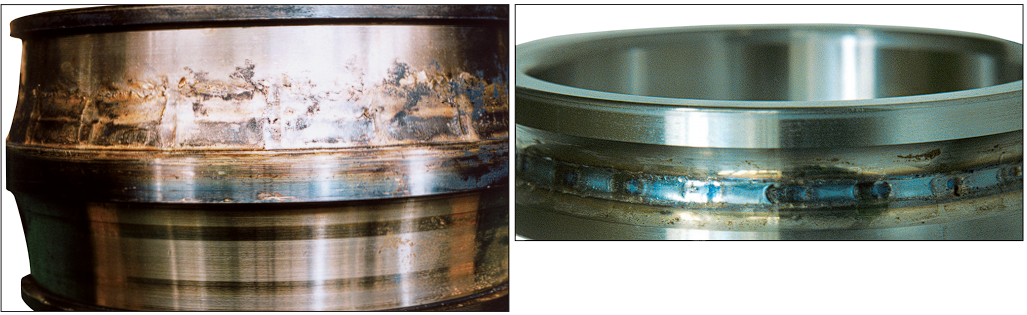
\includegraphics[width=\textwidth,height=\textheight,keepaspectratio]{superaquecimento_nsk}
\caption {Dano causado superaquecimento. Retirado de NSK, 2014.}
\label{superaquecimento_nsk}
\end{figure}


Corrosão eletrolítica diz respeito a formação de afundamentos sobre as pistas. Estes afundamentos transformam-se gradualmente em ondulações. A causa para isto é a corrente elétrica passando através dos corpos rolantes (NSK, 2014). A Figura~\ref{corrosao_eletrolitica_nsk} mostra a corrosão eletrolítica em na pista de um anel interno de um rolamento, com dano ampliado na foto para facilitação da visualização, bem como o dano em um anel externo. 

\begin{figure}[H]
\centering
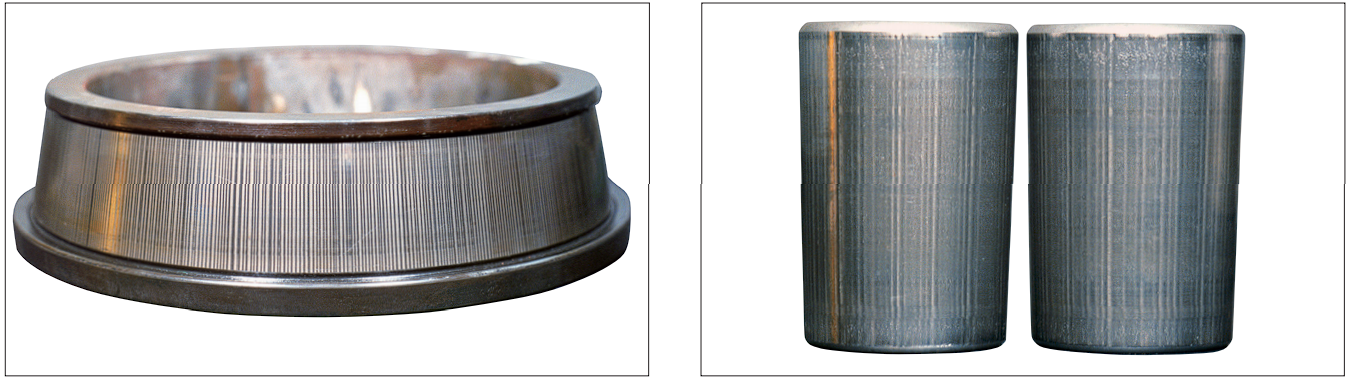
\includegraphics[width=\textwidth,height=\textheight,keepaspectratio]{corrosao_eletrolitica_nsk}
\caption {Corrosão eletrolítica em rolamentos. Retirado de NSK, 2014.}
\label{corrosao_eletrolitica_nsk}
\end{figure}


Oxidação e corrosão é uma falha que ocorre quando a superfície se torna parcial ou totalmente oxidada, e ocasionalmente óxido também surge ao longo das linhas do passo dos elementos rolantes. Causas para esta falha incluem condições inadequadas de armazenamento, embalagem inadequada, óleo protetivo insuficiente, penetração de água ou ácido, dentre outros elementos, ou, ainda, manuseio inadequado (NSK, 2014). A Figura~\ref{oxidacao_nsk} mostra um rolamento oxidado e corroído.

\begin{figure}[H]
\centering
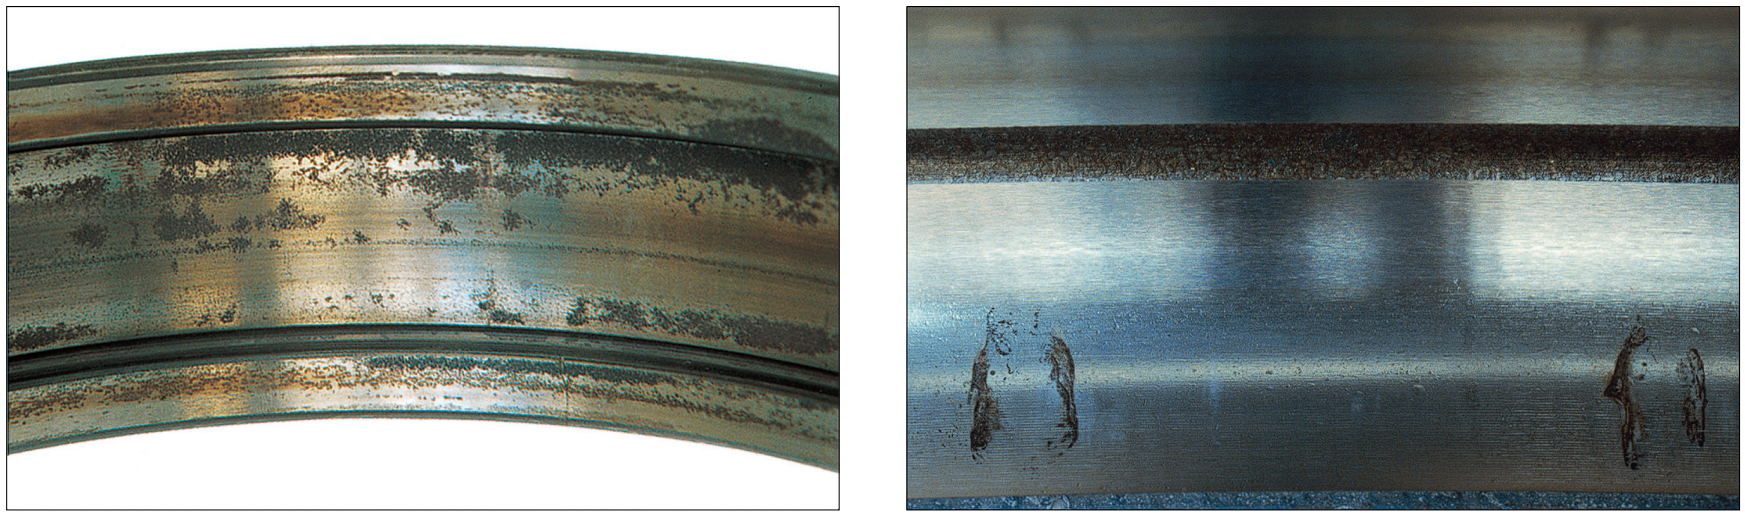
\includegraphics[width=\textwidth,height=\textheight,keepaspectratio]{oxidacao_nsk}
\caption {Rolamentos com oxidações e corrosões. Retirado de NSK, 2014.}
\label{oxidacao_nsk}
\end{figure}


Falhas na instalação têm como suas principais decorrências longo riscos na superfície das pistas ou dos elementos rolantes. As causas mais comuns são inclinação dos anéis ou impactos durante instalação ou remoção. A Figura~\ref{falha_instalacao_nsk} mostra um anel interno e externo com riscos decorrentes de falha de instalação.


\begin{figure}[H]
\centering
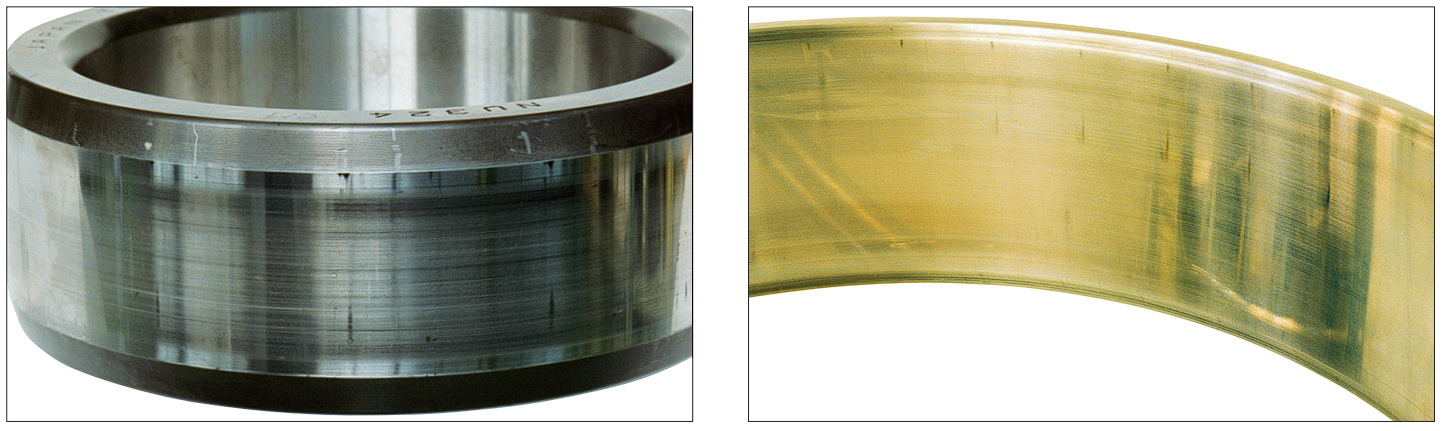
\includegraphics[width=\textwidth,height=\textheight,keepaspectratio]{falha_instalacao_nsk}
\caption {Rolamentos com falhas de instalação. Retirado de NSK, 2014.}
\label{falha_instalacao_nsk}
\end{figure}

Por fim, manchas e descoloração demonstram superfícies sem brilho, a superfície está fosca, rugosa ou eventualmente deformada, também estando coberta de pequenas depressões. As causas são infiltração de substância estranha ou mesmo lubrificação insuficiente (NSK, 2014). A Figura~\ref{manchas_nsk} mostra manchas e descoloração em rolamentos.

\begin{figure}[H]
\centering
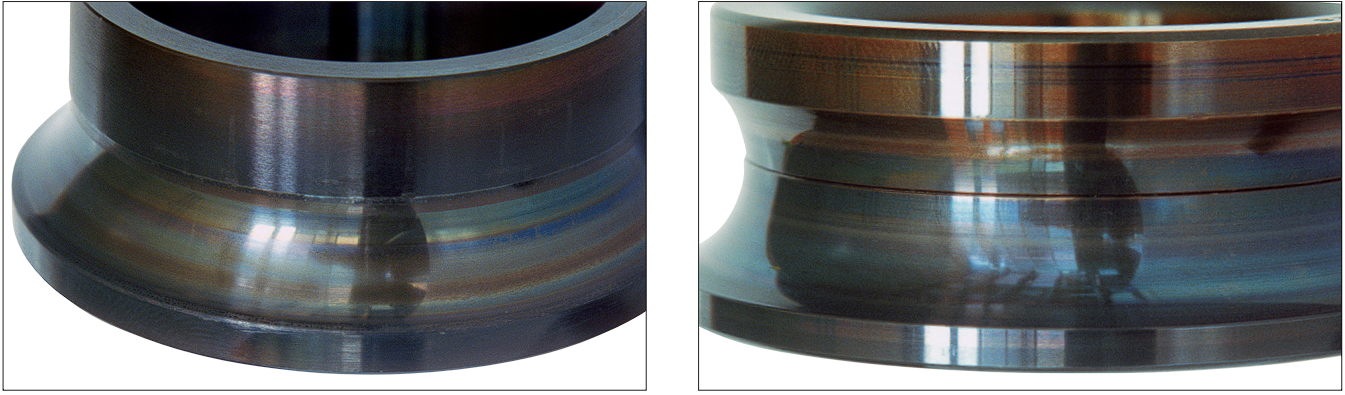
\includegraphics[width=\textwidth,height=\textheight,keepaspectratio]{manchas_nsk}
\caption {Manchas e descoloração em rolamentos. Retirado de NSK, 2014.}
\label{manchas_nsk}
\end{figure}

Ao verificar-se que houve o contato entre a superfície defeituosa de um elemento rolante e outra superfície sem defeito, o choque entre estes elementos causa um impulso que promove uma excitação tanto na máquina, quanto no rolamento. Assim, para detecção de falhas pode-se utilizar análise de vibrações, uma vez que os defeitos nos componentes dos rolamentos apresentam frequências características que podem ser calculadas a partir das especificações do rolamento. 


\subsection{\textbf{Frequências características de defeitos dos rolamentos}}

Assim, tem-se as seguintes fórmulas para o cálculo das frequências de defeitos dos vários  elementos que constituem um rolamento. 

FTF (\textit{fundamental train frequency}) indica a frequência de defeito na gaiola. 

\[FTF = \frac{fr}{2} \left ( 1 - \frac{d}{D} \,cos \, \theta \right )  \]

BPFI, indica a frequência de defeito na pista interna (\textit{ball pass frenquency of the inner race})

\[BPFI = \frac{N}{2}f_{r} \left ( 1 + \frac{d}{D} \,cos \, \theta \right )  \]

BPFO se trata do indicativo da frequência de defeito na pista externa (\textit{ball pass frequency of the outer race})

\[BPFO = \frac{N}{2}f_{r} \left ( 1 - \frac{d}{D} \,cos \, \theta \right )  \]

BSF, por sua vez, é o indicativo da frequência de defeito do elemento rolante (\textit{ball spin frequency}).

\[BSF = \frac{D}{2d}f_{r} \Bigg[  1 - \left ( \frac{d}{D} \,cos \, \theta \right ) ^{2}  \Bigg] \]

Onde, nestas fórmulas, temos $f_{r}$, que é a subtração da frequência de rotação da pista interna pela frequência de rotação da pista externa; $D$ é diâmetro primitivo, calculado a partir da soma do diâmetro externo pelo diâmetro interno e divisão do resultado por dois; $d$ é o diâmetro dos elementos rolantes; $N$ é o número de elementos rolantes; e, por fim, $\theta$ é o ângulo de contato.

Logo, a partir destas frequências características de defeito e das especificações dos rolamentos e de suas propriedades de trabalho - número de elementos rolantes, diâmetros, ângulo de contato e velocidade de rotação -, os componentes podem ser monitorados quanto ao surgimento de falhas.  

\section{\textbf{Fluroreto de polivinilideno}}

O fluoreto de polivinilideno, PVDF, é um fluoropolímero termoplátisco altamente inerte produzido a partir da polimerização do monômero chamado difluoretino (kabir et al., 2017). Em 1969 um pesquisador japonês, Dr. Heiji Kawai, descobriu altíssimos níveis de atividade piezoelétrica, muito superiores a qualquer polímero natural ou sintético conhecido, no fluoreto de polivinilideno (Marutake, 1995). Desde então, o PVDF vem tendo suas aplicações estudadas. O PVDF é um polímero semicristalino de cadeia longa, proveniente da unidade CH2-CF2. Esta unidade possui grande um grande momento do dipolo elétrico, de aproximadamente 7,56 x 10-30 C.m. Como estas unidades se alinham de maneira ordenada para uma configuração \textit{head-tail} superior à 90\%, o polímero apresenta um momento líquido do dipolo elétrico incomumente alto (Chatigny e Robb, 1987).

Decorrente desta descoberta o interesse no estudo do PVDF se dá, dentre outras caraterísticas, por suas propriedades piezo e piroelétricas. 

Piezoeletricidade é a capacidade de certos materiais, altamente polares, de alterar suas dimensões quando expostos a um campo elétrico, ou, inversamente, gerar sinal elétrico quando mecanicamente deformados (Halvorsen, 1986). A piezoeletricidade foi descoberta em 1880 pelos irmãos franceses Jacques e Pierre Curie, que a observaram em cristais de Quartzo (Manbacchi e Cobbold, 2011). Uma de suas primeiras aplicações tecnológicas foi feita por outro francês, Langevin, que desenvolveu um transmissor e receptor de quartzo para sons submarinos por volta de 1917 - o primeiro sonar (Halvorsen, 1986). Segundo Loussert et al., 2013, p.204 a piezoeletricidade se manifesta pela polarização da célula unitária com o aspecto de momento dipolar $\mu = q \,x \, d$, onde $q$ é a carga elétrica do dípolo e $d$ é a distância entre os centroides.  

As propriedades do PVDF, incluindo a piezoeletricidade, são altamente influenciadas pelo seu grau e tipo de estrutura de cristalina. Chatigny e Robb, 1987, fazem uma revisão relacionada ao processo de fabricação de filmes PVDF para obtenção das características desejadas em cada possível estrutura cristalina deste material. Nesta, afirmam que existem três formas distintas de estrutura cristalina no PVDF. A mais comum é centrossimétrica e não polar, obtida quando o polímero é resfriado a partir de seu ponto de derretimento, chamada de fase alfa. A deformação de grãos tipo alfa, com o stretching de filmes obtidos através de extrusão em temperaturas abaixo de 80ºC, faz com que as células unitárias se alinhem em planos paralelos, criando uma fase polar chamada de fase beta. Uma terceira configuração possível é a fase gama, que, ainda que polar, é intermediária em termos de centrossimetria entre as configurações de fases alfa e beta (Chatigny e Robb, 1987).

Para obtenção de níveis significativos de atividade piezoelétrica no material, o polímero em fase beta deve exposto a um campo elétrico de 500 a 1000KV/cm em temperaturas de 80 a 110ºC. Este processo é chamado de poling. O nível de atividade piezo depende do tempo de exposição a este campo elétrico, além da força do campo e da temperatura. Quando conduzido adequadamente, este processo provê orientação permanente para os dípolos no polímero (Chatigny e Robb, 1987). 

A Figura 20, abaixo, mostra as configurações alfa, gama e beta.

\begin{figure}[!htb]
\centering
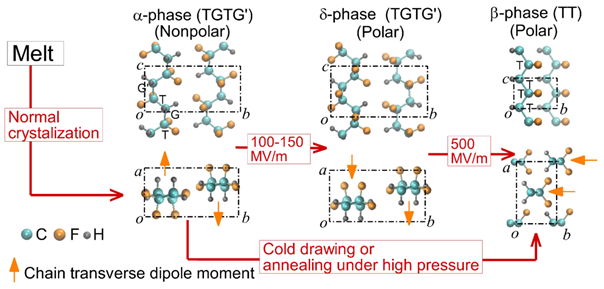
\includegraphics{Figura20}
\caption {Transições de fase do PVDF, induzidas por campo elétrico. Fases alfa, gama e beta. As células unitárias acima são mostradas nos planos ab e bc. O momento dípolo de cada cadeia polimérica é mostrado. Retirado de Wan e Bowen, 2017.}
\label{Figura20}
\end{figure}

Chatigny e Robb, 1987, descrevem um processo típico de preparação de um filme piezo pode ser resumido da seguinte forma:

\begin{enumerate}
	\item Extrusão do PVDF em filmes fase alfa; 
	\item Orientação, uniaxial ou biaxial, a 80ºC e uma relação de stretch de 4:5 para fase beta do filme;
	\item Deposição de eletrodos por algum de vários métodos;
	\item \textit{Poling} térmico a 600KV/cm a 100ºC, por aproximadamente trinta minutos.
\end{enumerate}

Durante este processo, os dípolos são alinhados relativos à direção do campo de \textit{poling}. Quando o filme piezo está operando em modo eletromecânico, o filme se alonga e contrai quando a polaridade dos campos se alterna. Quando operando de forma mecânico-elétrica, por sua vez, forças externas aplicadas produzem tensões de compressão e tração (Chatigny e Robb, 1987). 

Os filmes PVDF são flexíveis e leves, produzidos em uma variedade de espessuras e áreas. Algumas das vantagens dos filmes PVDF incluem elevada resistência química até temperaturas elevadas , 

Devemos considerar o filme piezoelétrico como um material dinâmico que desenvolve uma carga elétrica proporcional a mudança no stress mecânico. O piezo não opera em condições estáticas devido ao rápido decaimento da carga induzida, sendo sua constante de tempo determinada pela constante dielétrica do filme e sua resistência interna. 	Uma possível analogia, fornecida por Chatigny e Robb, 1987, é a de uma esponja despejando e absorvendo um fluido, conforme uma pressão externa é aplicada e então liberada. O filme age como uma esponja liberando uma carga elétrica na frequência que a deformação tem lugar. Uma vez que a deformação cessa, nenhuma carga é transferida. 

O PVDF é um material anisotrópico.  Suas propriedades elétricas, mecânicas e eletromecânicas diferem para as excitações elétricas e mecânicas nas diferentes direções. Desta forma, para uma tabulação sistemáticas das propriedades, utilizamos três eixos identificados por números: 1, correspondente ao comprimento; 2, correspondente a altura; e, por fim, 3, correspondente a espessura (Chatigny e Robb, 1987). 

Em relação a polarização do material, podemos dizer que tensões positivas são elásticas, enquanto tensões negativas são compressivas. Ação elétrica positiva é causada por um aumento na polarização e vice-versa. Para os filmes piezo, o eixo de polarização é sempre a espessura, uma vez que há alinhamento do campo nesta direção. O estresse mecânico, de qualquer forma, pode ser aplicado nas três direções. 

Usualmente utiliza-se algumas constantes para caracterizar as atividades de materiais piezoativos. 

A constante de acoplamento $K$, é a habilidade de trocar energia elétrica por energia mecânica e vice-versa. O quadrado da constante $K$ é igual a energia transformada dividida pela entrada total de energia. Assim, $K312$ é igual a energia elétrica transformada causadora de tensão mecânica ao longo do eixo 1, dividida pela energia elétrica total das faces eletrificadas paralelas ao eixo 3. 

A constante de tensão piezoelétrica, $d$, expressa a razão de tensão desenvolvida ao longo de um eixo específico aplicada paralelamente a um eixo específico. 

\[d_{31} = \frac{Tensao \,no \,eixo \,1}{Campo \,aplicado \,no \,eixo \,3} = \frac{m/m}{V/m} = \frac{m}{v} \]

Além disso

\[d_{31} = \frac{Carga \,por \,area \,de \,eletrodo}{Estresse \,aplicado \,no \,eixo \,1} = \frac{C/m^{2}}{N/m^{2}} = \frac{C}{N} \]

Outra constante é a constante de estresse piezoelétrico $g$, que expressa a razão do campo elétrico ao longo de um eixo especifico pelo estresse aplicado ao mesmo ou outro eixo. A constante g também expressa a tensão ao longo de um especifico pela carga elétrica por área unitária de eletrodos (Chattigny e Robb, 1987). Assim:

\[g_{33} = \frac{Campo \,aplicado \,ao \,longo \,do \,eixo \,3}{Estresse \,aplicado \,ao \,longo ,\do \,eixo \,3} = \frac{V/m}{N/m^{2}} = \frac{Vm}{N} \]

Além disso:

\[g_{33} = \frac{Tensao \,no \,eixo \,3}{Carga \,por \,area \,eletronica} = \frac{m/m}{C/m^{2}} = \frac{m^{2}}{C} \]

Também deve-se considerar a constante hidrostática piezoelétrica, $dh$, que representa a razão de carga de curto-circuito por área unitária da superfície dos eletrodos pelo estresse hidrostático aplicado igualmente ao longo dos três eixos. 

A constante piroelétrica, $p$, por sua vez, está ligada a natureza dos transdutores piezoelétricos. Estes absorvem energia térmica, aumentando assim a sua temperatura e induzindo sinais elétricos. Em filmes piezo o sinal de saída é proporcional à taxa de mudança de temperatura em vez de níveis de temperatura. A constante piroelétrica $p$, assim, relaciona a carga por unidade de área dos eletrodos pela unidade de troca de temperatura. Logo, $p = C/m^{2} K$.


\subsection{\textbf{Aplicações do Fluroreto de Polivinilideno}}

Dentre as distintas aplicações do PVDF, Xin et al., 2016, fizeram uma revisão de literatura quanto ao seu uso enquanto sensor de vibrações. Nesta, apresentam as seguintes aplicações:

\begin{itemize}
	\item PVDF como sensor aplicado a dispositivos médicos portáteis: com utilização em dispositivos VIVLAD, \textit{vibrating intravascular lung assist device}, a fim de auxiliar pacientes com problemas respiratórios crônicos; 
	 
	\item PVDF como sensor aplicados a monitoramento de saúde estrutural:

	\item PVDF como sensor aplicado a medição de vibrações em maquinário:

	\item PDVF como sensor aplicado em outras áreas:
	
\end{itemize}


%Descrever as aplicações do PVDF baseado na revisão de literatura feita por Xin, 2016.


\chapter{Materiais e métodos}

Para a realização dos experimentos serão utilizados dois rolamentos de rolos autocompensadores da NSK, modelo 21306CD. Este modelo apresenta como principais características uma alta capacidade de carga, gaiola de aço prensado e desalinhamento permissível entre $1^{\circ}$ e $2.5^{\circ}$. Esta categoria de rolamento foi escolhida pois possibilita uma maior facilidade para inserção manual de defeitos, o que possibilita a comparação entre os distintos estados de saúde do mesmo. 

As dimensões do rolamento escolhido são:

\begin{itemize}
	\item Número de elementos rolantes: 20 (10 por fileira)
	\item Diâmetro externo: 72\si{\mm}
	\item Diâmetro interno: 30\si{\mm}
	\item Limite de rotação: 4500 RPM lubrificado a graxa, 6000 RPM lubrificado a óleo
\end{itemize}

A Figura~\ref{Figura24} mostra o modelo do rolamento utilizado na bancada experimental.

\begin{figure}[H]
\centering
\includegraphics[width=\textwidth,height=100mm,keepaspectratio]{Figura24}
\caption {Rolamento utilizado na bancada de testes. Retirado de NSK, 2018.}
\label{Figura24}
\end{figure} 

Algumas das medidas necessárias para o cálculo das frequências características de defeito, a saber o ângulo de contato e o diâmetro dos elementos rolantes, não foram encontradas no manual do rolamento. Assim, a partir de pesquisa foi encontrado no site da NSK Japão um modelo CAD do mesmo, onde a partir deste calcularam-se os seguintes valores:

\begin{itemize}
	\item Diâmetro dos elementos rolantes: 10.1\si{\mm}
	\item Ângulo dos elementos rolantes: 14\textdegree
\end{itemize}

A Figura~\ref{angulo_de_contato} mostra o CAD do rolamento NSK 21306CD com vista frontal, estando com as marcações para mensuração do ângulo de contato. 

\begin{figure}[H]
\centering
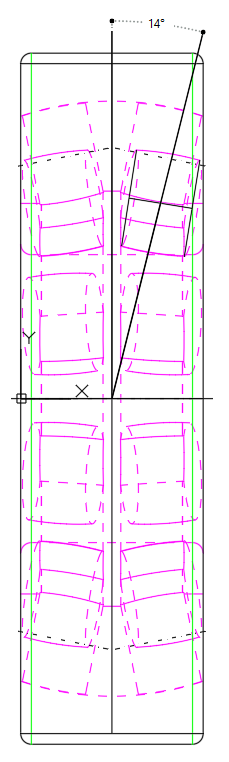
\includegraphics[width=\textwidth,height=150mm,keepaspectratio]{angulo_de_contato}
\caption {Ângulo de contato calculado a partir do modelo CAD disponibilizado pela NSK.}
\label{angulo_de_contato}
\end{figure} 

Já a Figura~\ref{diametro_rolamento} apresenta o diâmetro do elemento rolante, calculado a partir do raio de um dos elementos rolantes visto a partir da face direita do rolamento. 

\begin{figure}[H]
\centering
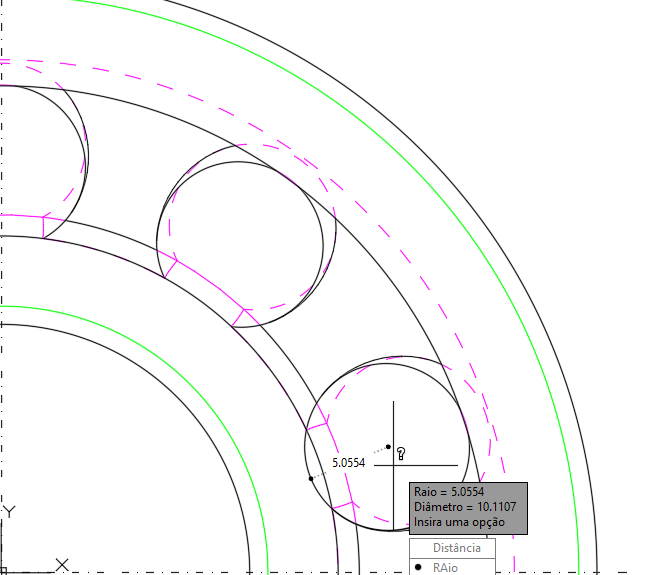
\includegraphics[width=\textwidth,height=100mm,keepaspectratio]{diametro_rolamento}
\caption {Diâmetro do elemento rolante calculado a partir do modelo CAD disponibilizado pela NSK.}
\label{diametro_rolamento}
\end{figure} 

As amostras do rolamento escolhido são novas e isentas de qualquer tipo de falha. Estas foram montadas em uma bancada experimental, construída para condução dos experimentos, onde terão terão registradas as suas assinaturas de vibração tanto no domínio da frequência, quanto do tempo para posterior análise. 

O aparato experimental é composto por um motoredutor cedido pela empresa parceira WEG/Cestari, com eixo motriz usinado e ligado à mancal de rolamento de empresa parceira NSK. A bancada possui em sua base um isolador de vibrações do tipo vibra-stop. A Figura~\ref{Figura22}, abaixo, mostra o projeto da bancada experimental. 

\begin{figure}[H]
\centering
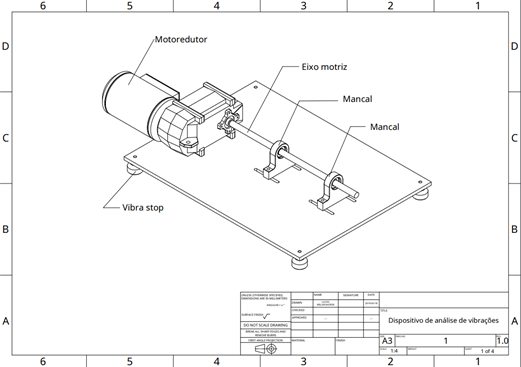
\includegraphics[width=\textwidth,height=\textheight,keepaspectratio]{Figura22}
\caption {Bancada experimental.}
\label{Figura22}
\end{figure}

Em relação a construção da bancada experimental, a mesma se deu durante o ano de 2019 no período imediatamente a pandemia de COVID-19. Foi utilizado um torno mecânico do IFSP Câmpus Guarulhos para usinagem do eixo, foi utilizada prensa afim de realizar o acoplamento dos mancais de rolamentos ao eixo usinado e posteriormente este foi ligado ao motoredutor. 

O motor utilizado na bancada de testes possui como características um torque de \SI{400}{\newton\metre}, velocidade de 1750 RPM com taxa de redução de 48,90 vezes, resultante em velocidade de saída para o eixo de 35,8 RPM.  

\begin{figure}[H]
\centering
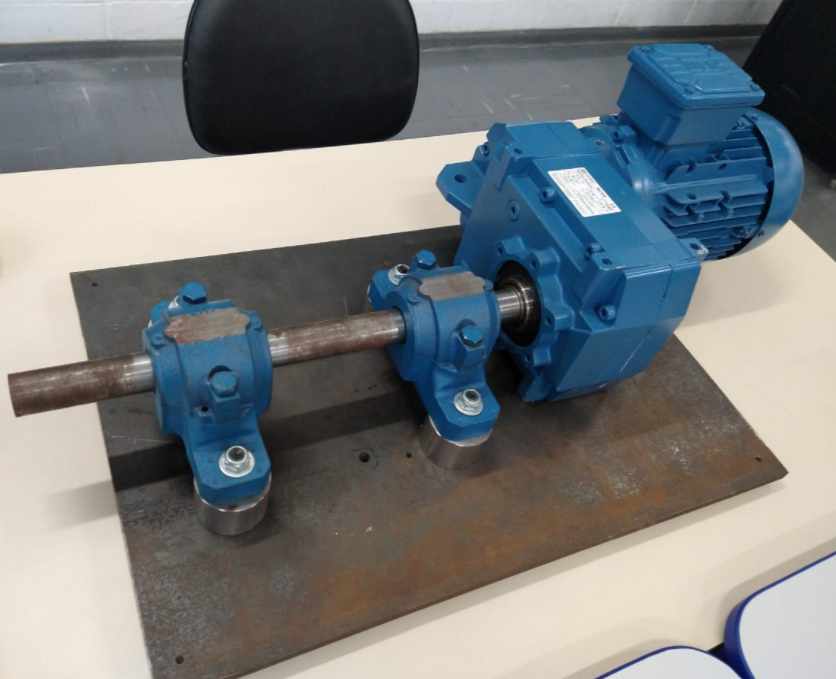
\includegraphics[width=\textwidth,height=\textheight,keepaspectratio]{bancada_de_testes}
\caption {Bancada experimental. Elaborado pelos autores.}
\label{bancada_de_testes}
\end{figure}

A partir destes dados, pode-se calcular com base nas frequências características de defeitos as frequências esperadas de defeito para o rolamento adotado no estudo. O diâmetro primitivo $D$ se dá por  


\[D = \frac{\SI{72}{\mm} \ + \SI{30}{\mm}}{2} = \SI{51}{\mm} \]  

Logo, para a \textit{Fundamental Train Frequency} temos, aproximadamente:

\[FTF = \frac{35}{2} \left ( 1 - \frac{10.1}{51} \,cos \, \ang{14} \right )  \ = \SI{~14}{{\hertz}} \]  

Para a \textit{Ball Pass Frequency of The Inner Race} temos, aproximadamente:

\[BPFI = \frac{10}{2}35 \left ( 1 + \frac{10.1}{51} \,cos \, \ang{14} \right )  \ = \SI{~208}{{\hertz}} \]


Para a \textit{Ball Pass Frequency of The Outer Race} temos, aproximadamente:

\[BPFO = \frac{10}{2}35 \left ( 1 - \frac{10.1}{51} \,cos \, \ang{14} \right )  \ = \SI{~141}{{\hertz}} \]

Por fim, para a \textit{Ball Spin Frequency} temos, aproximadamente:

\[BSF = \frac{51}{2*10.1}35 \Bigg[  1 - \left ( \frac{10.1}{51} \,cos \, \ang{14} \right ) ^{2}  \Bigg] \ = \SI{~85}{{\hertz}} \]


A partir destas frequências pode-se estimar as áreas para análise do sinal aquisitado, bem como realizar o tratamento e filtragem do sinal resultante do sensor afim de eliminação de interferências eletromagnéticas. 

Serão aquisitados sinais de todas as amostras com defeitos, com a utilização de sensores fabricados com o polímero PVDF, com terminais que permitem a medição da sua diferença de potencial, quando estes estiverem sujeitos a um esforço mecânico. 

Tendo em vista se tratarem de sensores de alta impedância, se faz necessário isolamento elétrico, afim de mitigar as interferências da fase da rede elétrica e de sinais de rádio incidentes sobre o local de testes, bem como tratamento da tensão resultante de esforço mecânico através de amplificação do sinal. 

Para tanto, utiliza-se um encapsulamento construído em alumínio, onde se acomoda o filme PVDF, além de amplificador operacional Texas Instruments TL-082. 

Tal amplificador de instrumentação foi utilizado por possuir ganho de até .... 

A Figura~\ref{Figura21} mostra o sensor de vibração. 

\begin{figure}[H]
\centering
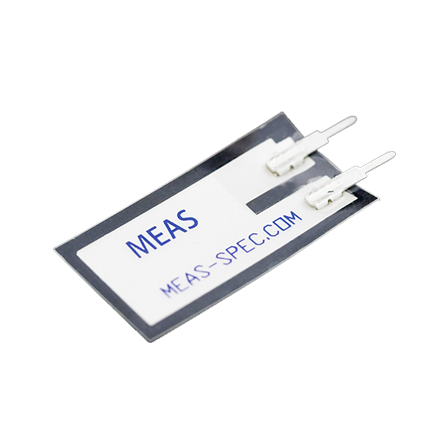
\includegraphics[width=\textwidth,height=100mm,keepaspectratio]{Figura21}
\caption {Sensor de vibração piezoelétrico.}
\label{Figura21}
\end{figure} 

A montagem dos sensores se deu em um encapsulamento de alumínio. Estes são acoplados com cola acrílica, afim de que não ocorra amortecimento da vibração devido ao elemento colante. Uma vez montado o aparato, os sinais decorrentes da vibração são aquisitados para posterior comparação com os sinais característicos dos rolamentos sem defeitos afim de que se determine a severidade da falha.

\begin{figure}[H]
\centering
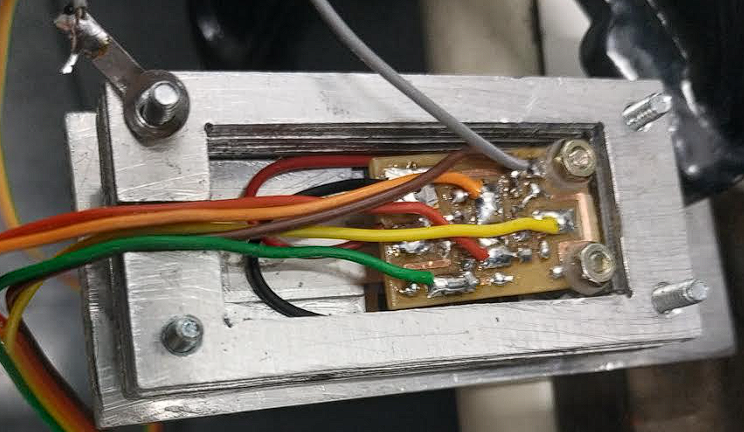
\includegraphics[width=\textwidth,height=\textheight,keepaspectratio]{encapsulamento_sensor}
\caption {Sensor de vibração piezoelétrico.}
\label{encapsulamento_sensor}
\end{figure} 

Os modelos matemáticos de identificação de frequências características de defeitos serão utilizados para a análise dos sinais no domínio do tempo e da frequência, que terão a finalidade de calibragem dos níveis de alarme. A análise se dará através de nível RMS, Curtose e Transformada rápida de Fourier.  

Para a análise, utilizam-se as plataformas Pandas, construída na linguagem de programação python e Octave. São ferramentas gratuitas e de código aberto. 

%Por fim, os custos dos sensores fabricados em PVDF serão calculados e comparados com os equipamentos atualmente disponíveis para aferição do custo vs benefício, visando com esta ação reduzir a ocorrência de falhas catastróficas, que são um grande risco tanto para a segurança dos operadores de máquinas quanto para a saúde financeira das empresas pela parada não programada da produção.

A análise dos resultados obtidos se dará à luz da revisão bibliográfica e comparativamente com os resultados encontrados em outros artigos. 

\chapter{Conclusões e próximos passos}

A partir da revisão bibliográfica realizada e dos passos já tomados, pretende-se o início dos experimentos entre Julho e Setembro de 2021. 

Com os dados colhidos, será possível avaliar o sinal e definir

A Tabela 1 mostra o cronograma de desenvolvimento.

\begin{table}[H]
\centering
\caption{Cronograma de desenvolvimento}
\resizebox{\textwidth}{!}
{\begin{tabular}{|l|l|l|l|l|l|l|}

\hline
\multirow{2}{*}{Atividades }                                                  & \multicolumn{6}{l|}{2019}                                  \\ 
\cline{2-7}
                                                                              & Julho & Agosto & Setembro & Outubro & Novembro & Dezembro  \\ 
\hline
Finalização de revisão bibliográfica~ ~ ~ ~ ~                                 & X     & X      &          &         &          &           \\ 
\hline
Término da montagem da bancada experimental~ ~ ~ ~ ~                          & X     & X      &          &         &          &           \\ 
\hline
Finalização dos testes dos circuitos e sistema de aquisição de dados~ ~ ~ ~ ~ &       & X      & X        & X       &          &           \\ 
\hline
Testes experimentais~ ~ ~ ~ ~~                                                &       & X      & X        & X       &          &           \\ 
\hline
Análise de resultados~ ~ ~ ~ ~                                                &       &        &          & X       &          &           \\ 
\hline
Qualificação~ ~ ~ ~ ~                                                         &       &        &          & X       & X        &           \\ 
\hline
Submissão de artigo~ ~ ~ ~ ~                                                  &       &        &          &         & X        &           \\ 
\hline
Apresentação em Simpósio/Congresso~ ~ ~ ~ ~                                   &       &        &          &         & X        &           \\ 
\hline
Escrita da dissertação~ ~ ~ ~ ~                                               &       &        & X        & X       & X        &           \\ 
\hline
Defesa~ ~ ~ ~ ~~                                                              &       &        &          &         & X        &           \\ 
\hline
Ajustes e entrega da versão final~ ~ ~ ~ ~                                    &       &        &          &         &          & X         \\
\hline
\end{tabular}}
\label{tab:ExemploDeTabela1}
\source{Os autores, 2019}
\end{table}



% ----------------------------------------------------------
% ELEMENTOS PÓS-TEXTUAIS
% ----------------------------------------------------------
\postextual
% ----------------------------------------------------------

% ----------------------------------------------------------
% Referências bibliográficas
% ----------------------------------------------------------

%\bibliography{referencias}


\begin{thebibliography}{9}

\bibitem{ABNT1994}
  ABNT, Associação Brasileira de Normas Técnicas.
  \textbf{NBR 5462: Confiabilidade e mantenabilidade}.
  Rio de Janeiro, 1994, 37p.

\bibitem{BARCOHEN2002}
  BAR-COHEN, Y.
  \textbf{Electroactive Polimers as Artificial Muscles: a review}.
  Journal of Spacecraft and Rockets, 39 (8), pg. 322-328, 2002.
    
\bibitem{CNI2019}
 CNI, Confederação Nacional das Indústrias.
  \textbf{Perfil da Indústria Brasileira}.
  Brasil, 2019. Disponível em: Disponível em: https://industriabrasileira.portaldaindustria.com.br/grafico/total/producao/industria-total. Acesso em: 07/06/2021.
 
\bibitem{FUKADA2000}
  FUKADA E.
  \textbf{History and recent progress in piezoeletric polymers}.
  IEE transactions on ultrasonics, ferroelectrics, and frequency control, vol. 47, 2000.

\bibitem{HARRIS1991}
  HARRIS, T. A.
  \textbf{Rolling Bearing Analysis}.
  3ªed. New York, John Wiley \& Sons, EEUU, 1991.

\bibitem{JUVINALL1991}
  JUVINALL, R.C., MARSHEK, K.M.
  \textbf{Fundamentals of Machine Component Design}.
  2ª ed. New York, John Wiley \& Sons, EEUU, 1991.

\bibitem{kardec2009}
  KARDEC, Alan; NASCIF, Júlio.
  \textbf{Manutenção: Função Estratégica}.
  3.ed. Rio de Janeiro: Qualitymark: Petrobras, 2009.

\bibitem{LANG2006}
  LANG S. B.; MUENSIT S.
  \textbf{Review of some lesser-known applications of piezoelectric and pyroeletric polymers}.
  Journal of applied physics. v. 85, p.125- 134, 2006.

\bibitem{Nepomuceno1989}
 NEPOMUCENO, Lauro Xavier.
  \textbf{Técnicas de Manutenção Preditiva}.
  Editora Edgard.1 ed. São Paulo: Blücher, 1989. 1 v.

\bibitem{Rao2008}
 RAO, Singiresu S.
  \textbf{Mechanical Vibrations}.
  4.ed. São Paulo: Pearson Prentice Hall, 2008.
  
\bibitem{SILVA2009}
    SILVA, ALINE BRUNA da.
  \textbf{Processamento, caracterização e determinação do perfil de polarização do Poli(fluoreto de vinilideno)}.
  São Carlos: UFSCar, 2009.

\bibitem{Slack2008}
 SLACK, Nigel.
  \textbf{Administração da Produção}.
  2.ed. São Paulo: Atlas, 2008.
 
\bibitem{WISNIEWSKI2002}
    WISNIEWSKI, C; FERREIRA, G. F. L.; FARIA, R. M.; GIACOMETTI, J. A.
  \textbf{Stable and metastable ferroelectric polarization analysed by the ramp voltage technique.}
  Proceedings of 11th International Symposium on Electrets. Melbourne: Piscatway, p.215 – 218, 2002.




  

\end{thebibliography}


% ----------------------------------------------------------
% Glossário
% ----------------------------------------------------------
%
% Consulte o manual da classe abntex2 para orientações sobre o glossário.
%
%\glossary

% ----------------------------------------------------------
% Apêndices
% ----------------------------------------------------------


% ---


% ----------------------------------------------------------
% Anexos
% ----------------------------------------------------------

% ---
% Inicia os anexos
% ---
\begin{anexosenv}

% Imprime uma página indicando o início dos anexos
%\partanexos

\end{anexosenv}





\end{document}
